\documentclass[english,11pt]{beamer}

\DeclareMathOperator{\Cov}{Cov}
\DeclareMathOperator{\Var}{Var}
\DeclareMathOperator{\E}{\mathbb{E}}
\DeclareMathOperator{\Proba}{\mathbb{P}}

\newcommand{\Covb}[2]{\ensuremath{\Cov\!\left[#1,#2\right]}}
\newcommand{\Eb}[1]{\ensuremath{\E\!\left[#1\right]}}
\newcommand{\Pb}[1]{\ensuremath{\Proba\!\left[#1\right]}}
\newcommand{\Varb}[1]{\ensuremath{\Var\!\left[#1\right]}}

% norm
\newcommand{\norm}[1]{\| #1 \|}

\newcommand{\indep}{\rotatebox[origin=c]{90}{$\models$}}





\usepackage{mathptmx,amsmath,amssymb,graphicx,bibentry,bbm,babel,ragged2e}

\makeatletter

\newcommand{\noun}[1]{\textsc{#1}}
\newcommand{\jitem}[1]{\item \begin{justify} #1 \end{justify} \vfill{}}
\newcommand{\sframe}[2]{\frame{\frametitle{#1} #2}}

\newenvironment{centercolumns}{\begin{columns}[c]}{\end{columns}}
%\newenvironment{jitem}{\begin{justify}\begin{itemize}}{\end{itemize}\end{justify}}

\usetheme{Warsaw}
\setbeamertemplate{footline}[text line]{}
\setbeamertemplate{headline}{}
\setbeamercolor{structure}{fg=purple!50!blue, bg=purple!50!blue}

\setbeamersize{text margin left=15pt,text margin right=15pt}

\setbeamercovered{transparent}


\@ifundefined{showcaptionsetup}{}{%
 \PassOptionsToPackage{caption=false}{subfig}}
\usepackage{subfig}

\usepackage[utf8]{inputenc}
\usepackage[T1]{fontenc}

\usepackage{multirow}


\makeatother

\begin{document}





\title{Towards integrated urban models for sustainable policies}

\author{J.~Raimbault$^{1,2,3\ast}$\\
\texttt{j.raimbault@ucl.ac.uk}
}


\institute{$^{1}$CASA, UCL\\
$^{2}$UPS CNRS 3611 Complex Systems Institute Paris\\
$^{3}$UMR CNRS 8504 G{\'e}ographie-cit{\'e}s
}


\date{Urban Analytics Tongji Workshop\\
July 3rd 2019
}

\frame{\maketitle}


% Juste Raimbault holds a PhD from University Paris 7, under the supervision of Arnaud Banos (Géographie-cités) and Florent Le Nechet (LVMT), studying modeling the co-evolution of transportation networks and territories. With an interdisciplinary background in Complex Systems, his work is situated at the interface of Geography and Computer Science. He is currently a Research Fellow at CASA, UCL, where he studies the coupling of microsimulation models with land-use transport interaction models, and a Post-doctoral researcher at ISC-PIF where he develops model exploration and calibration methods and contributes to the development of the OpenMOLE platform.


%\AtBeginSection[]
%{
%	\frame{
%		\tableofcontents[currentsection, hideallsubsections]
%	}
%	\addtocounter{framenumber}{-1}
%}


% no need for outline
%\sframe{Outline}{
%\tableofcontents
%}
%\section{Introduction}


\sframe{Scientific background}{


\begin{columns}

	\begin{column}{0.5\textwidth}
	

	\begin{center}
	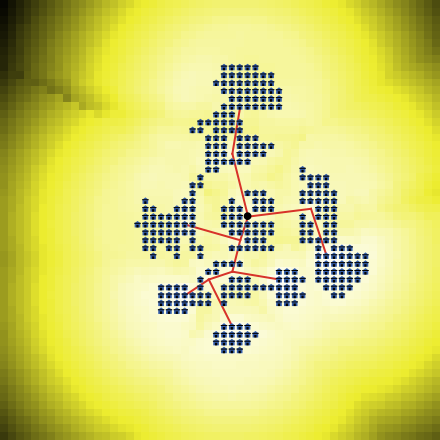
\includegraphics[width=0.85\textwidth]{figures/intro_RBD_lattice.png}
	\end{center}
	
	%\footnotesize
\textit{Hybrid urban morphogenesis model}
	
	\bigskip
	
	\nocite{raimbault2014hybrid}
	
	\tiny
 
 \justify
 
 Raimbault, J., Banos, A., \& Doursat, R. (2014, June). A Hybrid Network/Grid Model of Urban Morphogenesis and Optimization. In 4th International Conference on Complex Systems and Applications (pp. 51-60).
	

	\end{column}
	\vrule{}
	\begin{column}{0.5\textwidth}

	\begin{center}
	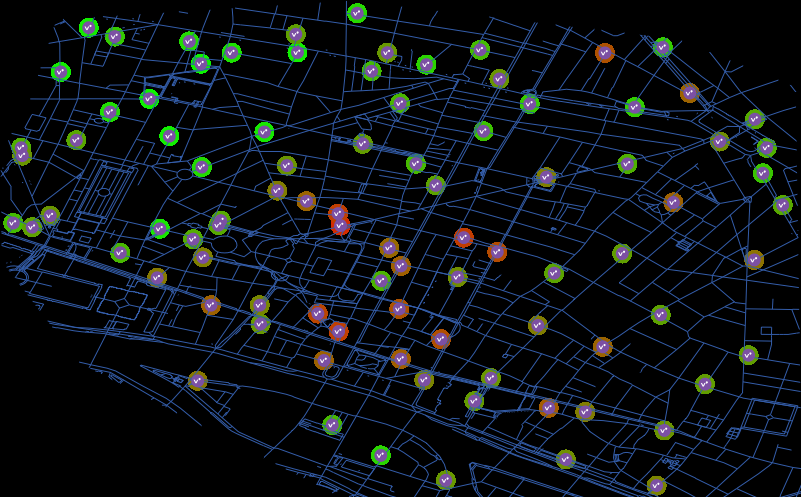
\includegraphics[width=\textwidth]{figures/velib.png}
		\end{center}
		
\textit{Agent-based modeling of bike-sharing}

\bigskip

\tiny
\justify


 Raimbault, J. (2015). User-based solutions for increasing level of service in bike-sharing transportation systems. In Complex Systems Design \& Management (pp. 31-44). Springer, Cham.

\nocite{raimbault2015user}

	\end{column}


\end{columns}

}





\sframe{Interactions between networks and territories}{

\justify

\begin{center}
\includegraphics[width=0.45\linewidth]{figures/accessp_withbridge_prd_EN.png}
\hspace{0.1cm}
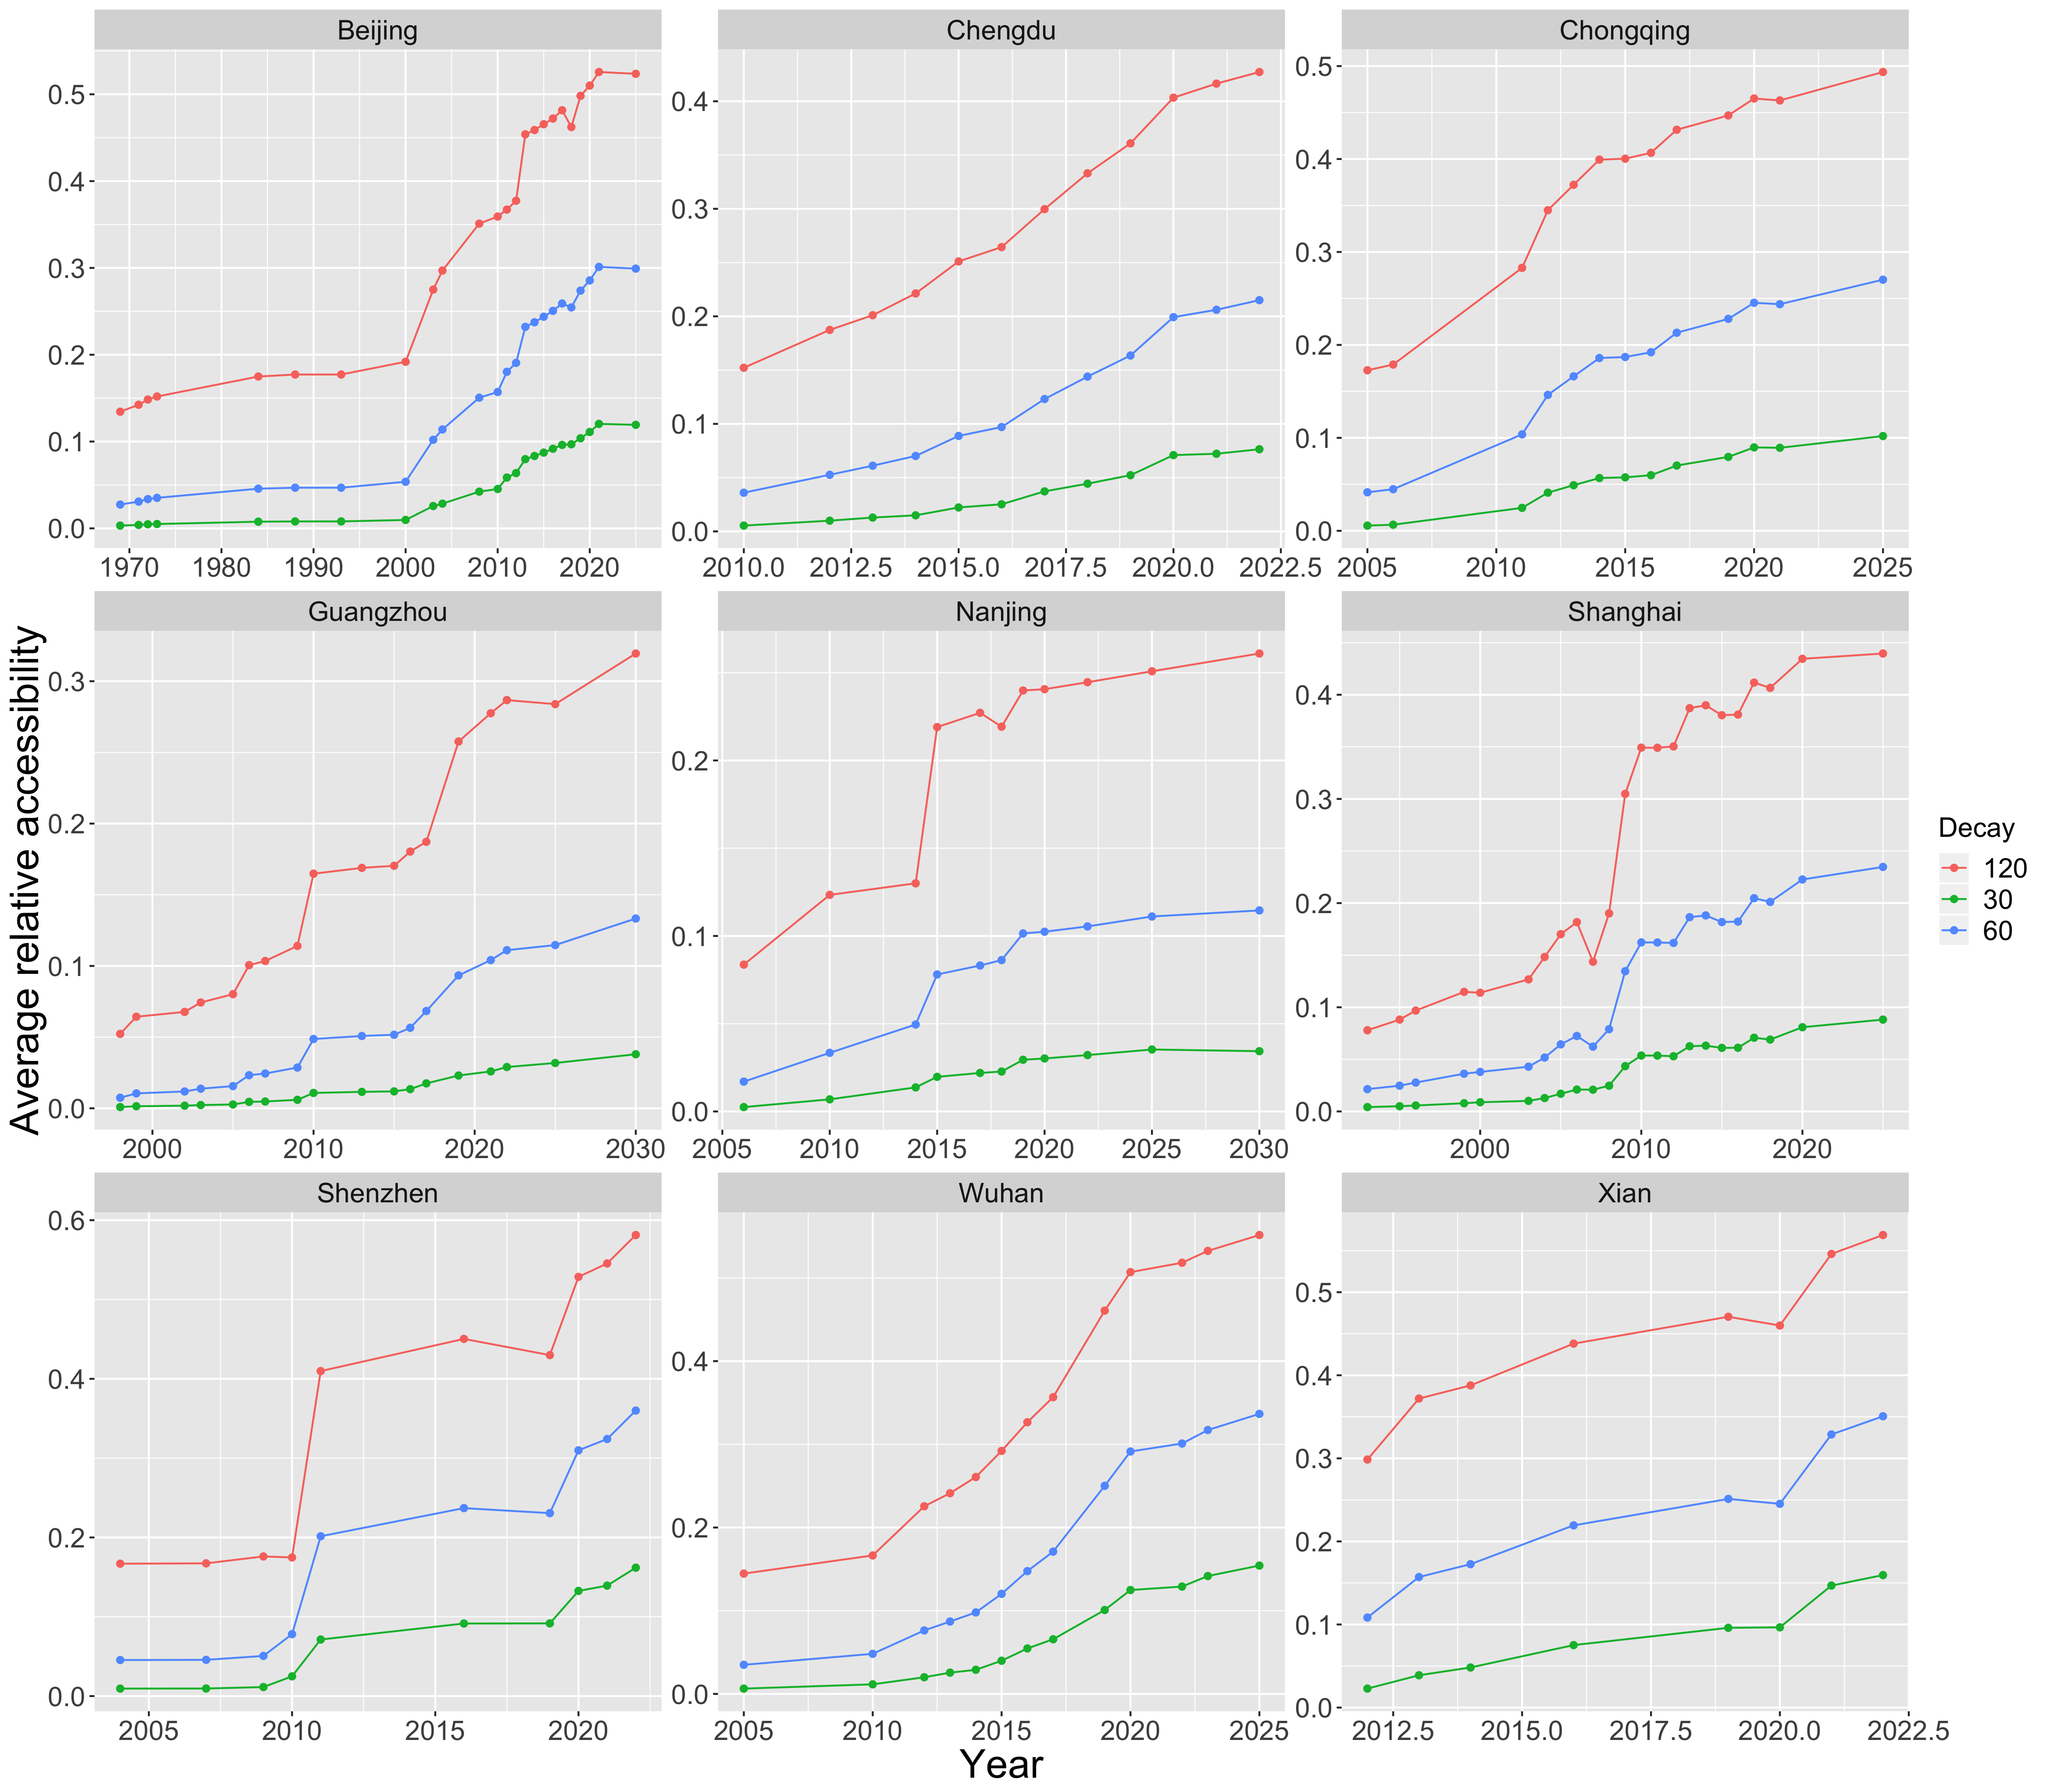
\includegraphics[width=0.52\linewidth]{figures/avgaccess_facet.png}

\end{center}

\medskip

%\vspace{-0.5cm}

%\begin{justify}
\textit{Accessibility as part of complex processes of co-evolution between transportation networks and territories.}

%\end{justify}

\nocite{raimbault2018evolving}

\medskip

\tiny

Raimbault, J. (2019). Evolving accessibility landscapes: mutations of transportation networks in China. In Aveline-Dubach, N., ed. \textit{Pathways of sustainable urban development across China - the cases of Hangzhou, Datong and Zhuhai}, pp 89-108. Imago. ISBN:978-88-94384-71-0

}



\sframe{Modeling the co-evolution of networks and territories}{
	
	
	\textbf{Macroscopic scale:}
	\begin{itemize}
		\item Interaction models between cities including networks		
		$\rightarrow$ \textit{Demonstration of network effects; exploration\\
		 of interaction regimes}
	\end{itemize}

	\bigskip

	\textbf{Mesoscopic scale:}
	\begin{itemize}
		\item Urban morphogenesis model coupling urban form and network growth
		
		 $\rightarrow$ \textit{Complementarity of multiple processes; calibration at the first and second order}
		\item Exploration of a model including transportation governance
	\end{itemize}

	
}



\sframe{Mesoscopic models: morphogenesis}{


% - complementarité de multiples heuristiques de croissance de reseau
% - calibration au premier et second ordre
% - Lutecia : vers des modèles plus complexes


\footnotesize

%Relation entre forme et fonction (morphogenèse) comme paradigme pour modéliser la co-évolution à l'échelle mésoscopique.

%\smallskip

%\begin{columns}
%\begin{column}{0.55\textwidth}

%\footnotesize

\vspace{-0.8cm}

\justify
\textit{A morphogenesis model with reaction-diffusion and multi-modeling of network growth: complementarity of heuristics, calibration for Europe on forms and their correlations}

\smallskip

\begin{center}
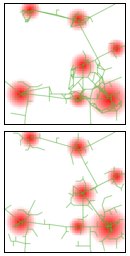
\includegraphics[width=0.25\linewidth,height=0.6\textheight]{figures/meso-nwgrowth.png}
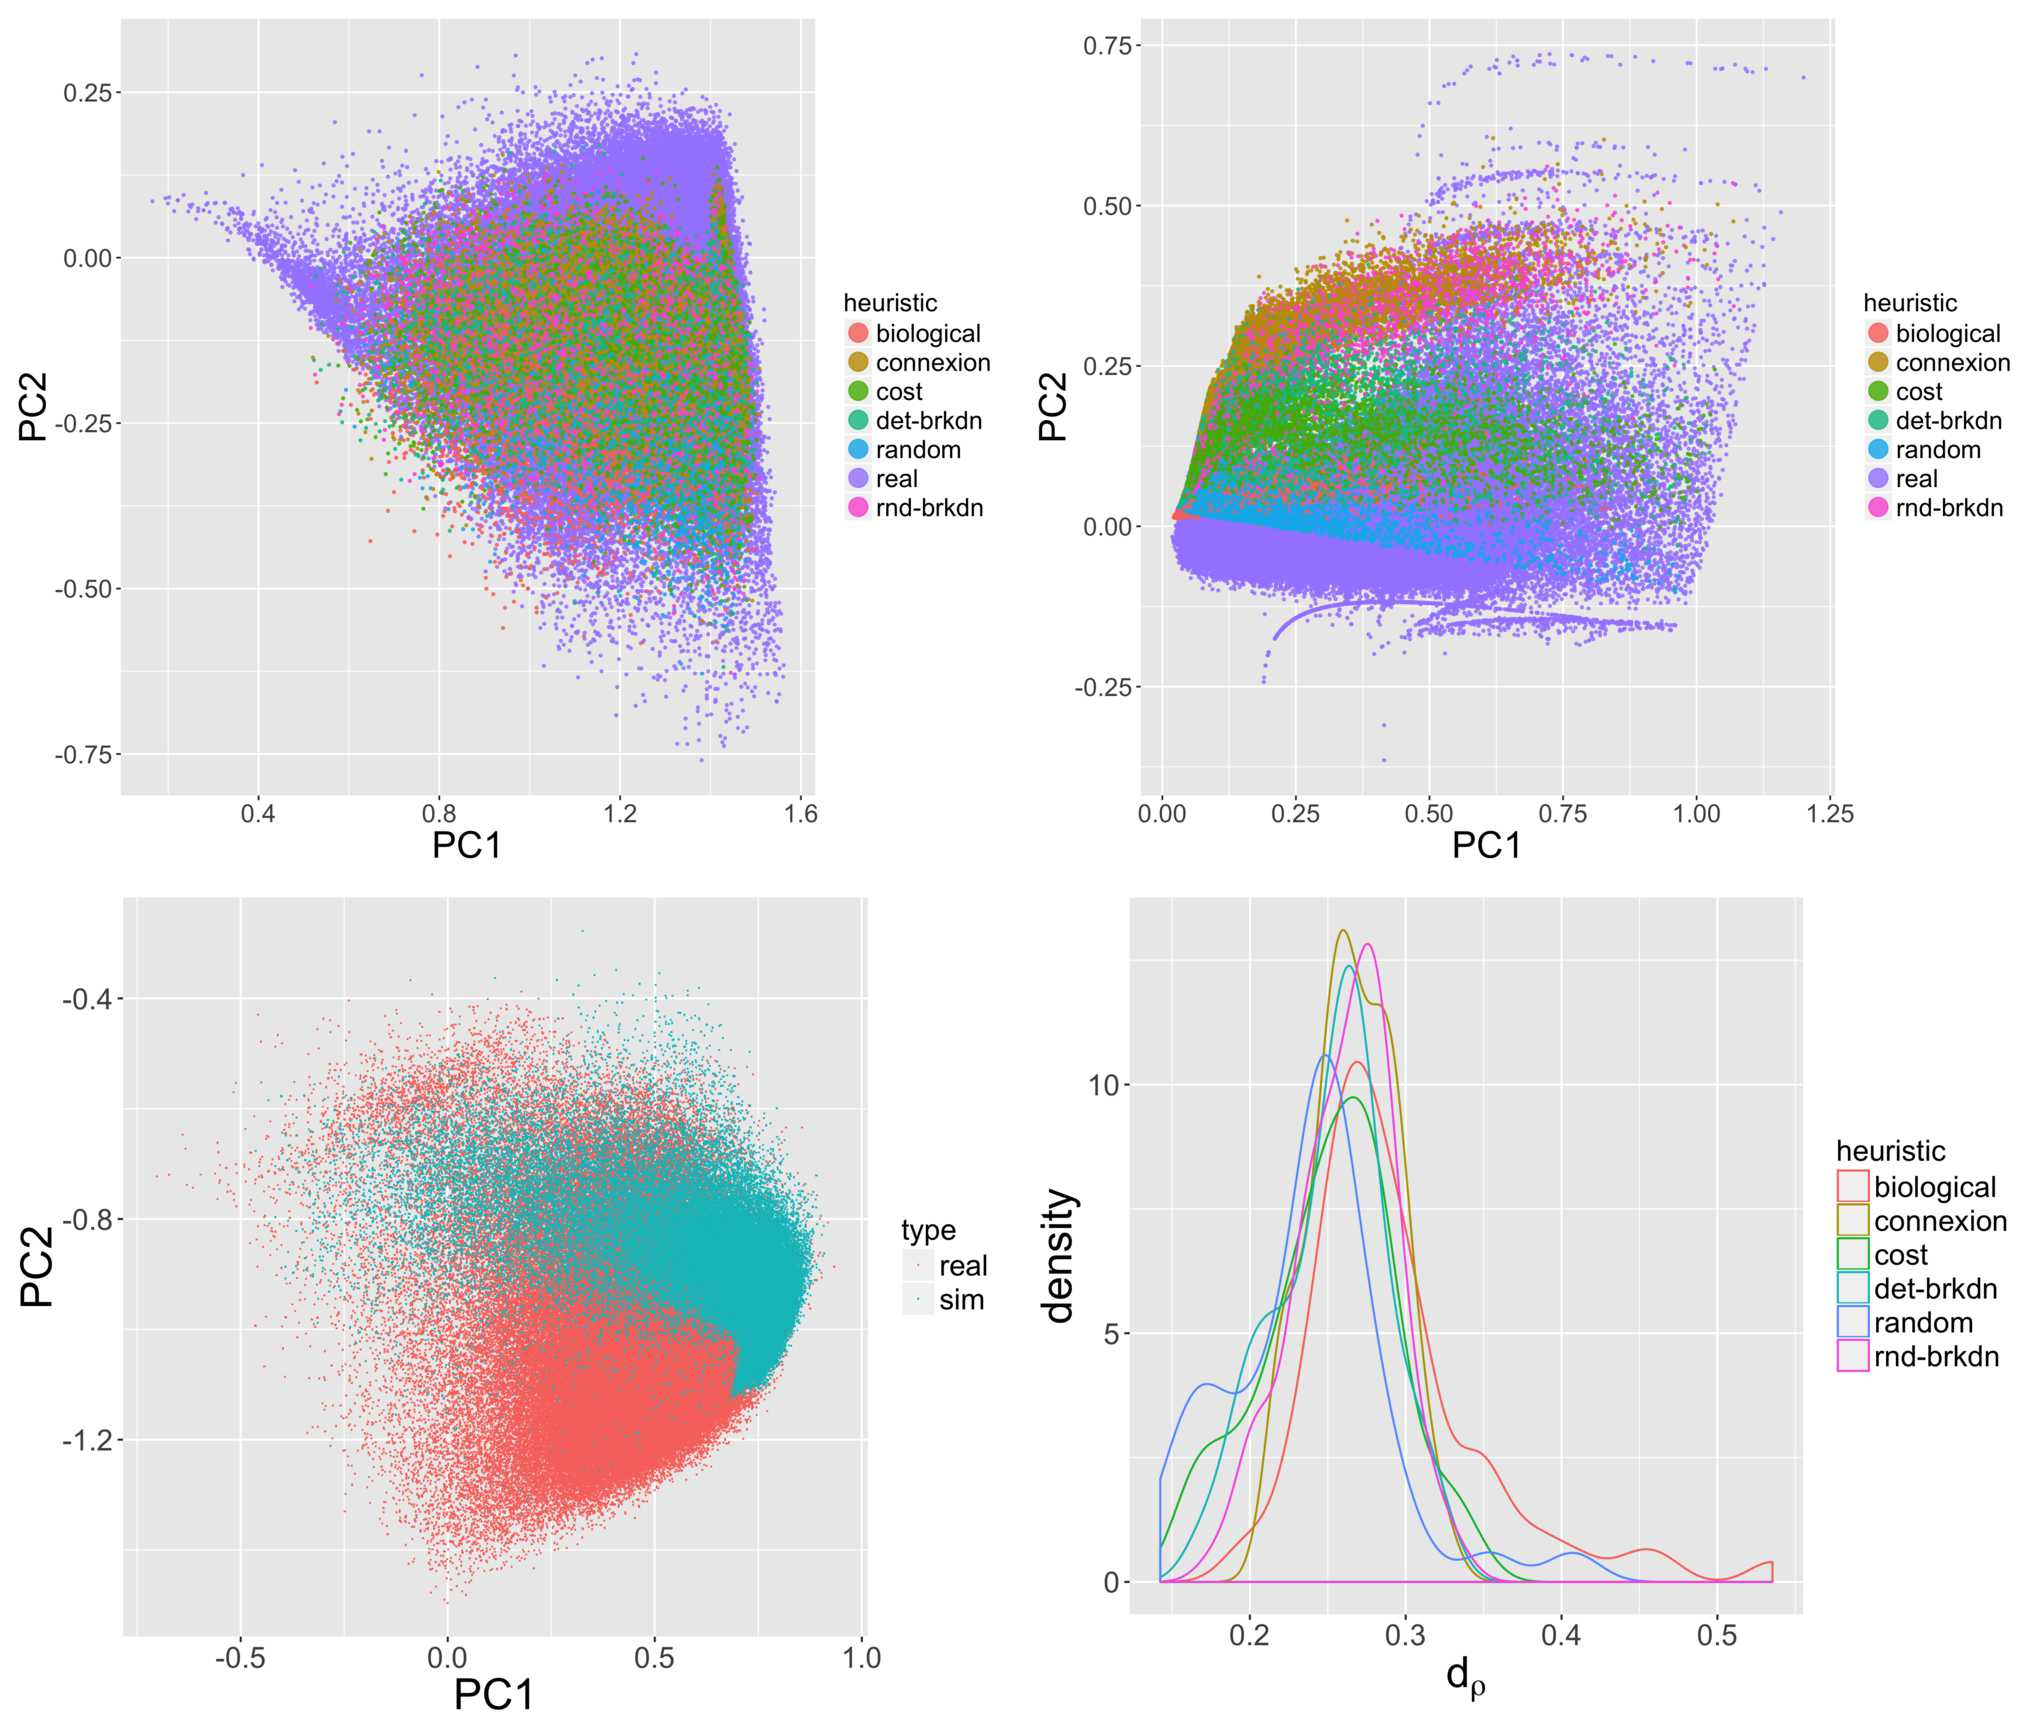
\includegraphics[width=0.6\linewidth,height=0.6\textheight]{figures/meso-calib.jpg}
\end{center}


\smallskip

\tiny

Raimbault, J. (2018). Calibration of a density-based model of urban morphogenesis. PloS one, 13(9), e0203516.

\nocite{raimbault2018calibration}

\smallskip

Raimbault, J. (2019). An urban morphogenesis model capturing interactions between networks and territories. In The Mathematics of Urban Morphology (pp. 383-409). Birkhäuser, Cham.

\nocite{raimbault2019urban}

%\smallskip

%Raimbault, J. (2018). Multi-modeling the morphogenesis of transportation networks. In Artificial Life Conference Proceedings (pp. 382-383).
}







\sframe{Macroscopic interaction model}{

\textit{System of cities interaction model including network evolution; production of multiple co-evolution regimes and calibration for France.}

\medskip

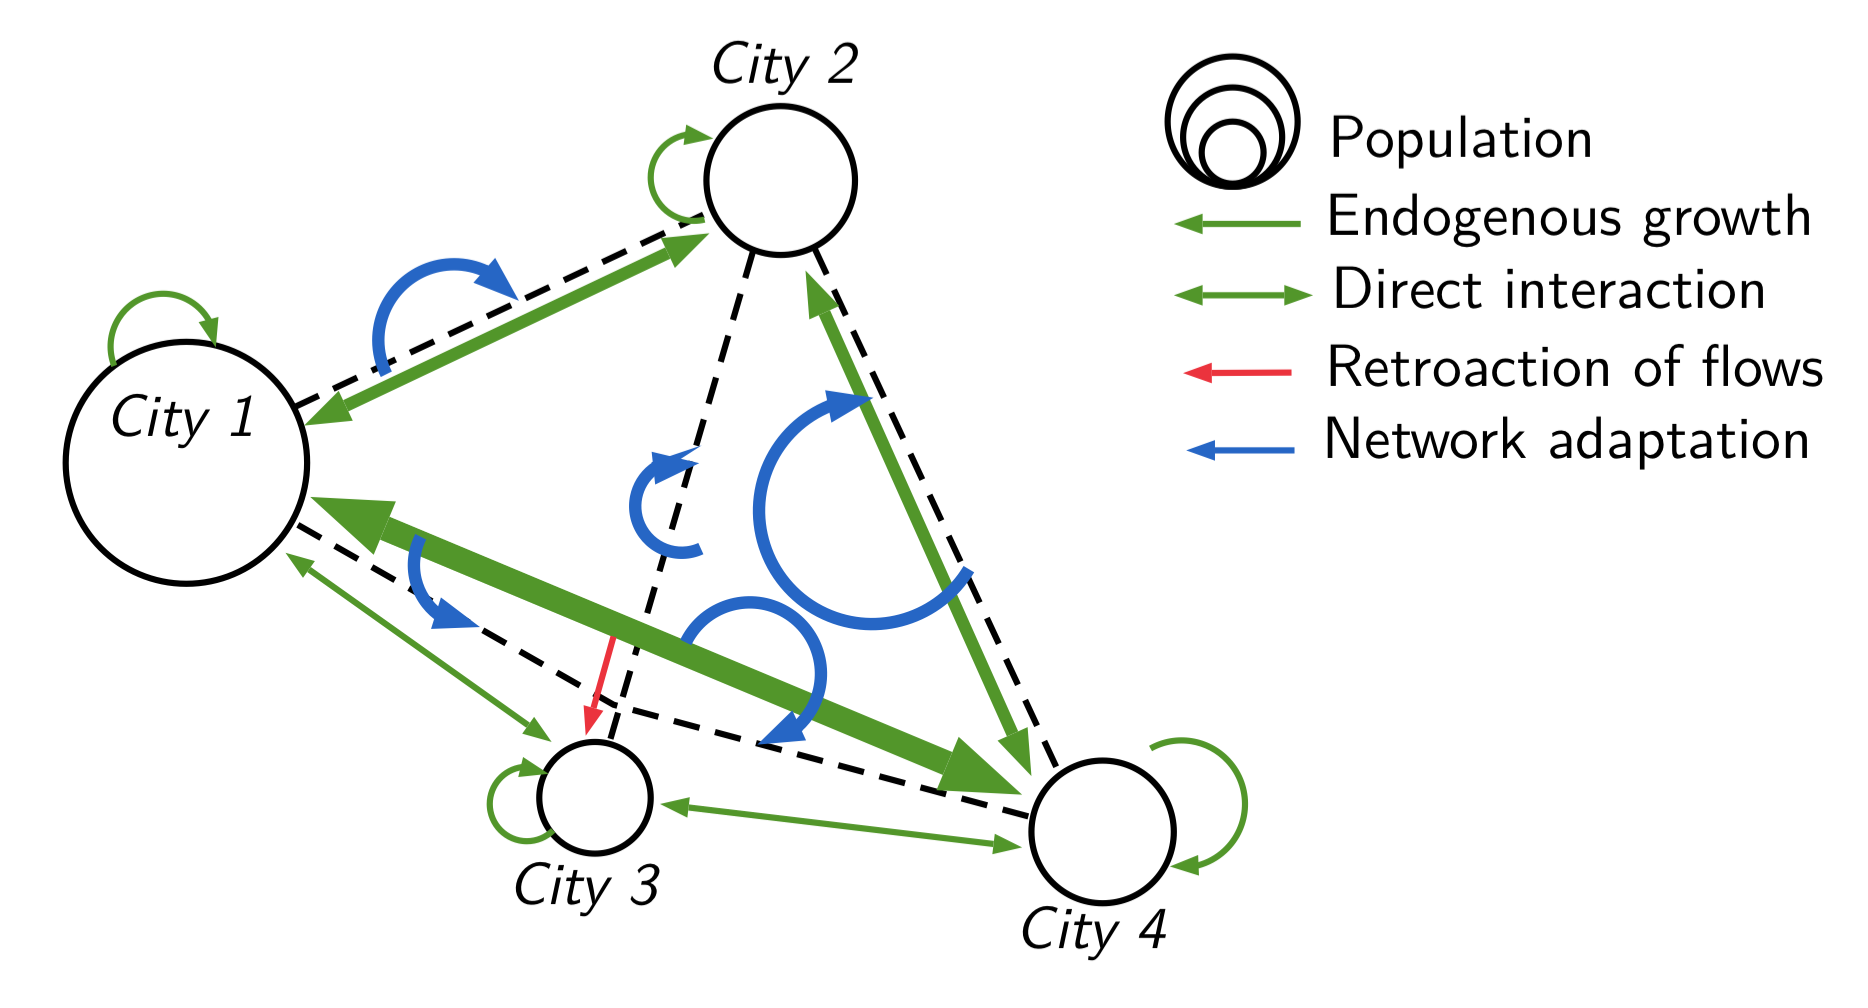
\includegraphics[width=0.6\textwidth]{figures/macrocoevol_en.png}
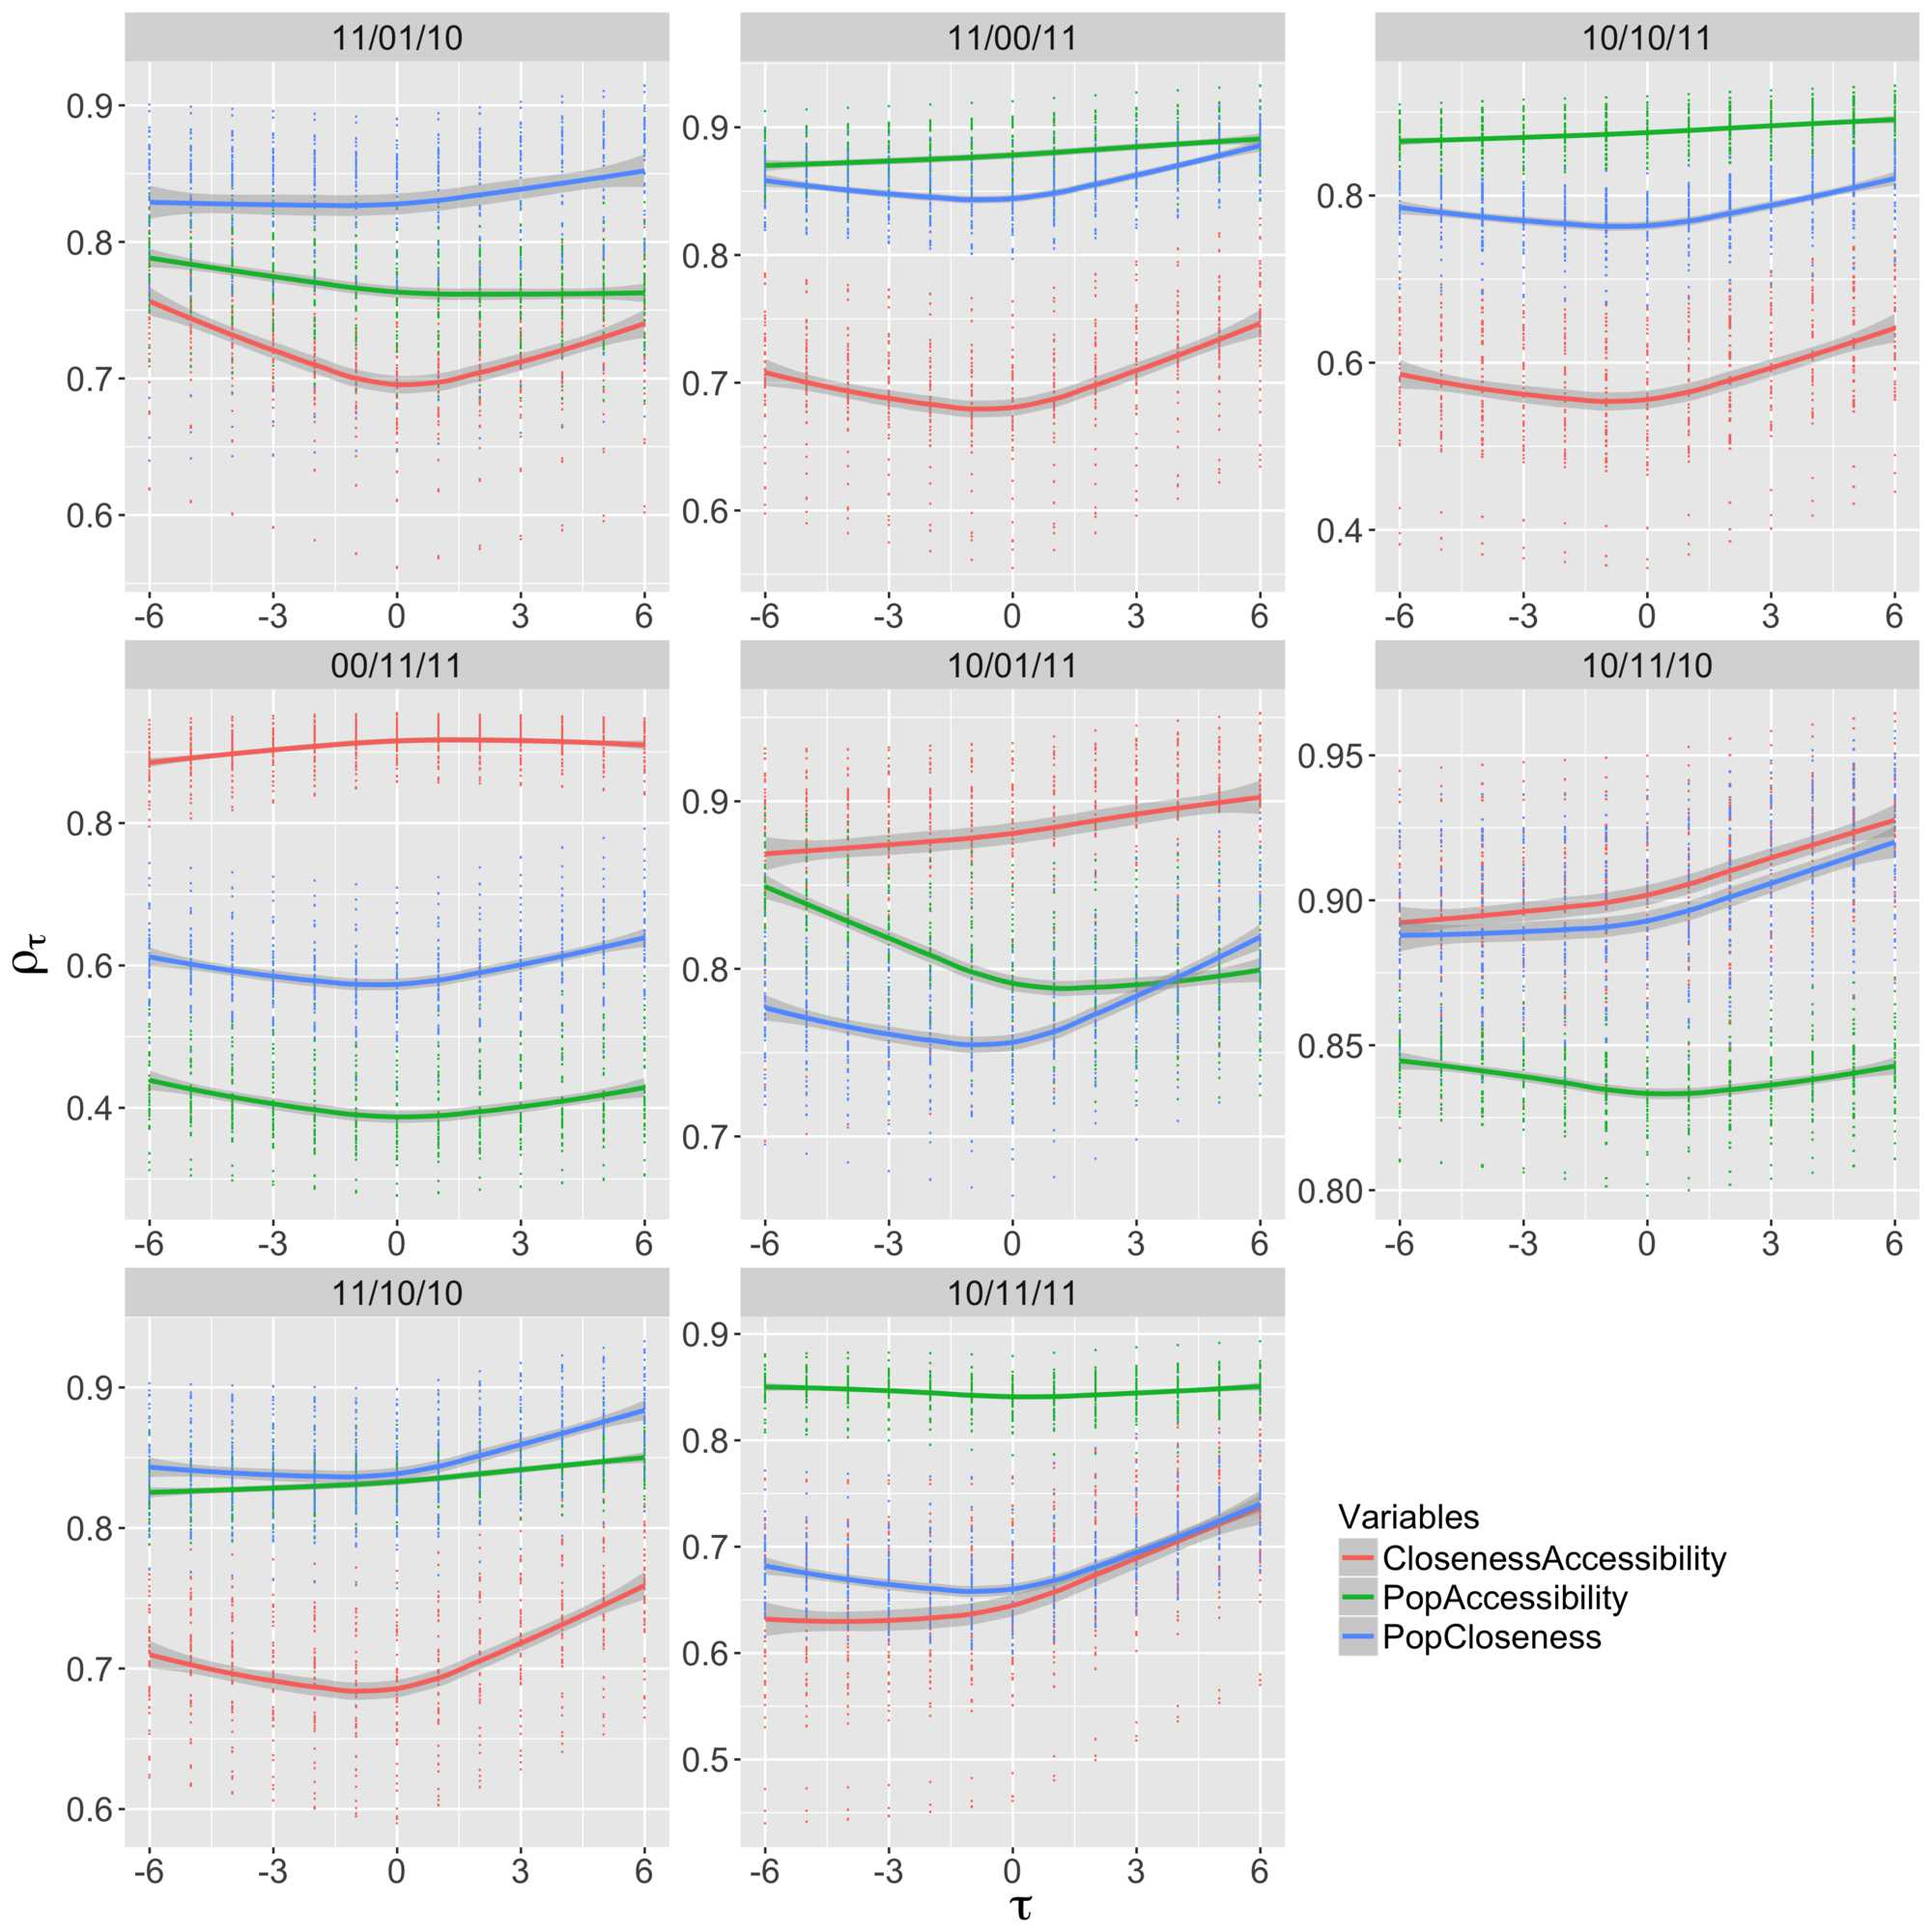
\includegraphics[width=0.39\linewidth]{figures/6-2-2-fig-macrocoevol-correlations.jpg}


\nocite{raimbault2018indirect}
\nocite{raimbault2019modeling}


\bigskip

\tiny

Raimbault, J. (2018). Indirect evidence of network effects in a system of cities. Environment and Planning B: Urban Analytics and City Science, 2399808318774335.

\smallskip

Raimbault, J. (2019). Modeling the co-evolution of cities and networks. In Niel, Z., Rozenblat, C., eds. \textit{Handbook of Cities and Networks}, Edwar Elgar Publishing, \textit{in press}.


}




\sframe{Towards integrated models}{


Types of integrations for urban models:

\medskip

\begin{itemize}
	\item Horizontal integration (interdisciplinarity)
	\item Vertical integration (multi-scale)
	\item Knowledge domain integration
\end{itemize}

%\begin{columns}
%
%	\begin{column}{0.32\textwidth}
%
%	\textit{Horizontal integration (interdisciplinarity)}
%
%	\begin{center}
%	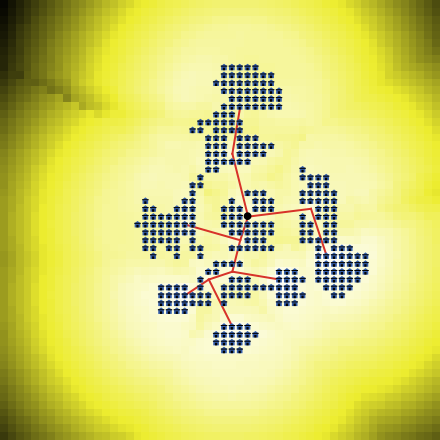
\includegraphics[width=0.58\textwidth]{figures/intro_RBD_lattice.png}
%	\end{center}
%
%	\end{column}
%	\vrule{}
%	\begin{column}{0.32\textwidth}
%
%	\textit{Vertical integration (multi-scale)}
%
%	\begin{center}
%	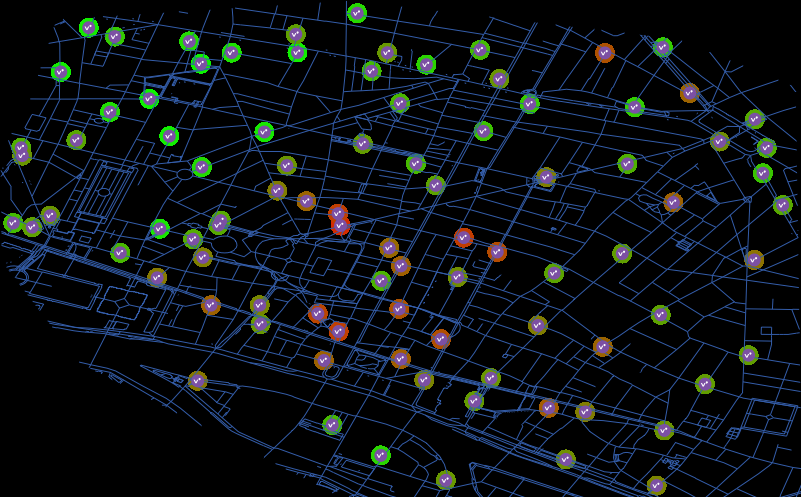
\includegraphics[width=0.8\textwidth]{figures/velib.png}
%		\end{center}
%
%	\end{column}
%	\vrule{}
%	\begin{column}{0.32\textwidth}
%
%	\textit{Knowledge domain integration}
%
%	\begin{center}
%	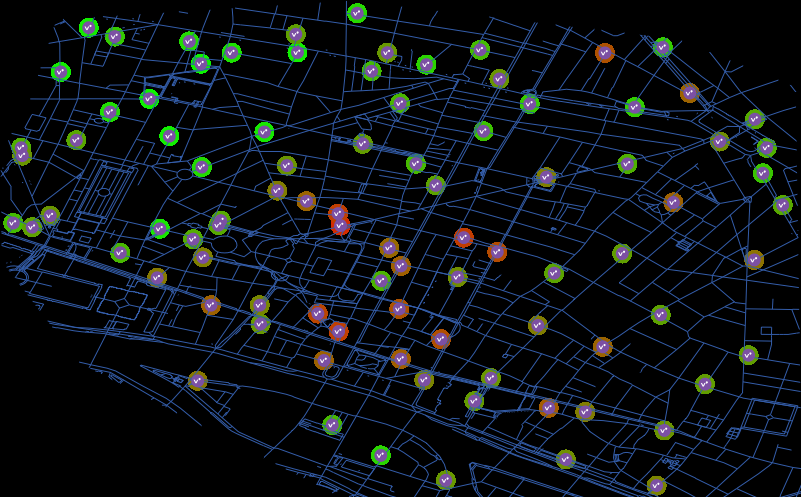
\includegraphics[width=0.8\textwidth]{figures/velib.png}
%		\end{center}
%
%	\end{column}
%\end{columns}



}



\sframe{Horizontal integration: interdisciplinarity}{

\textit{Complementary modeling approaches}

\medskip

\begin{center}
	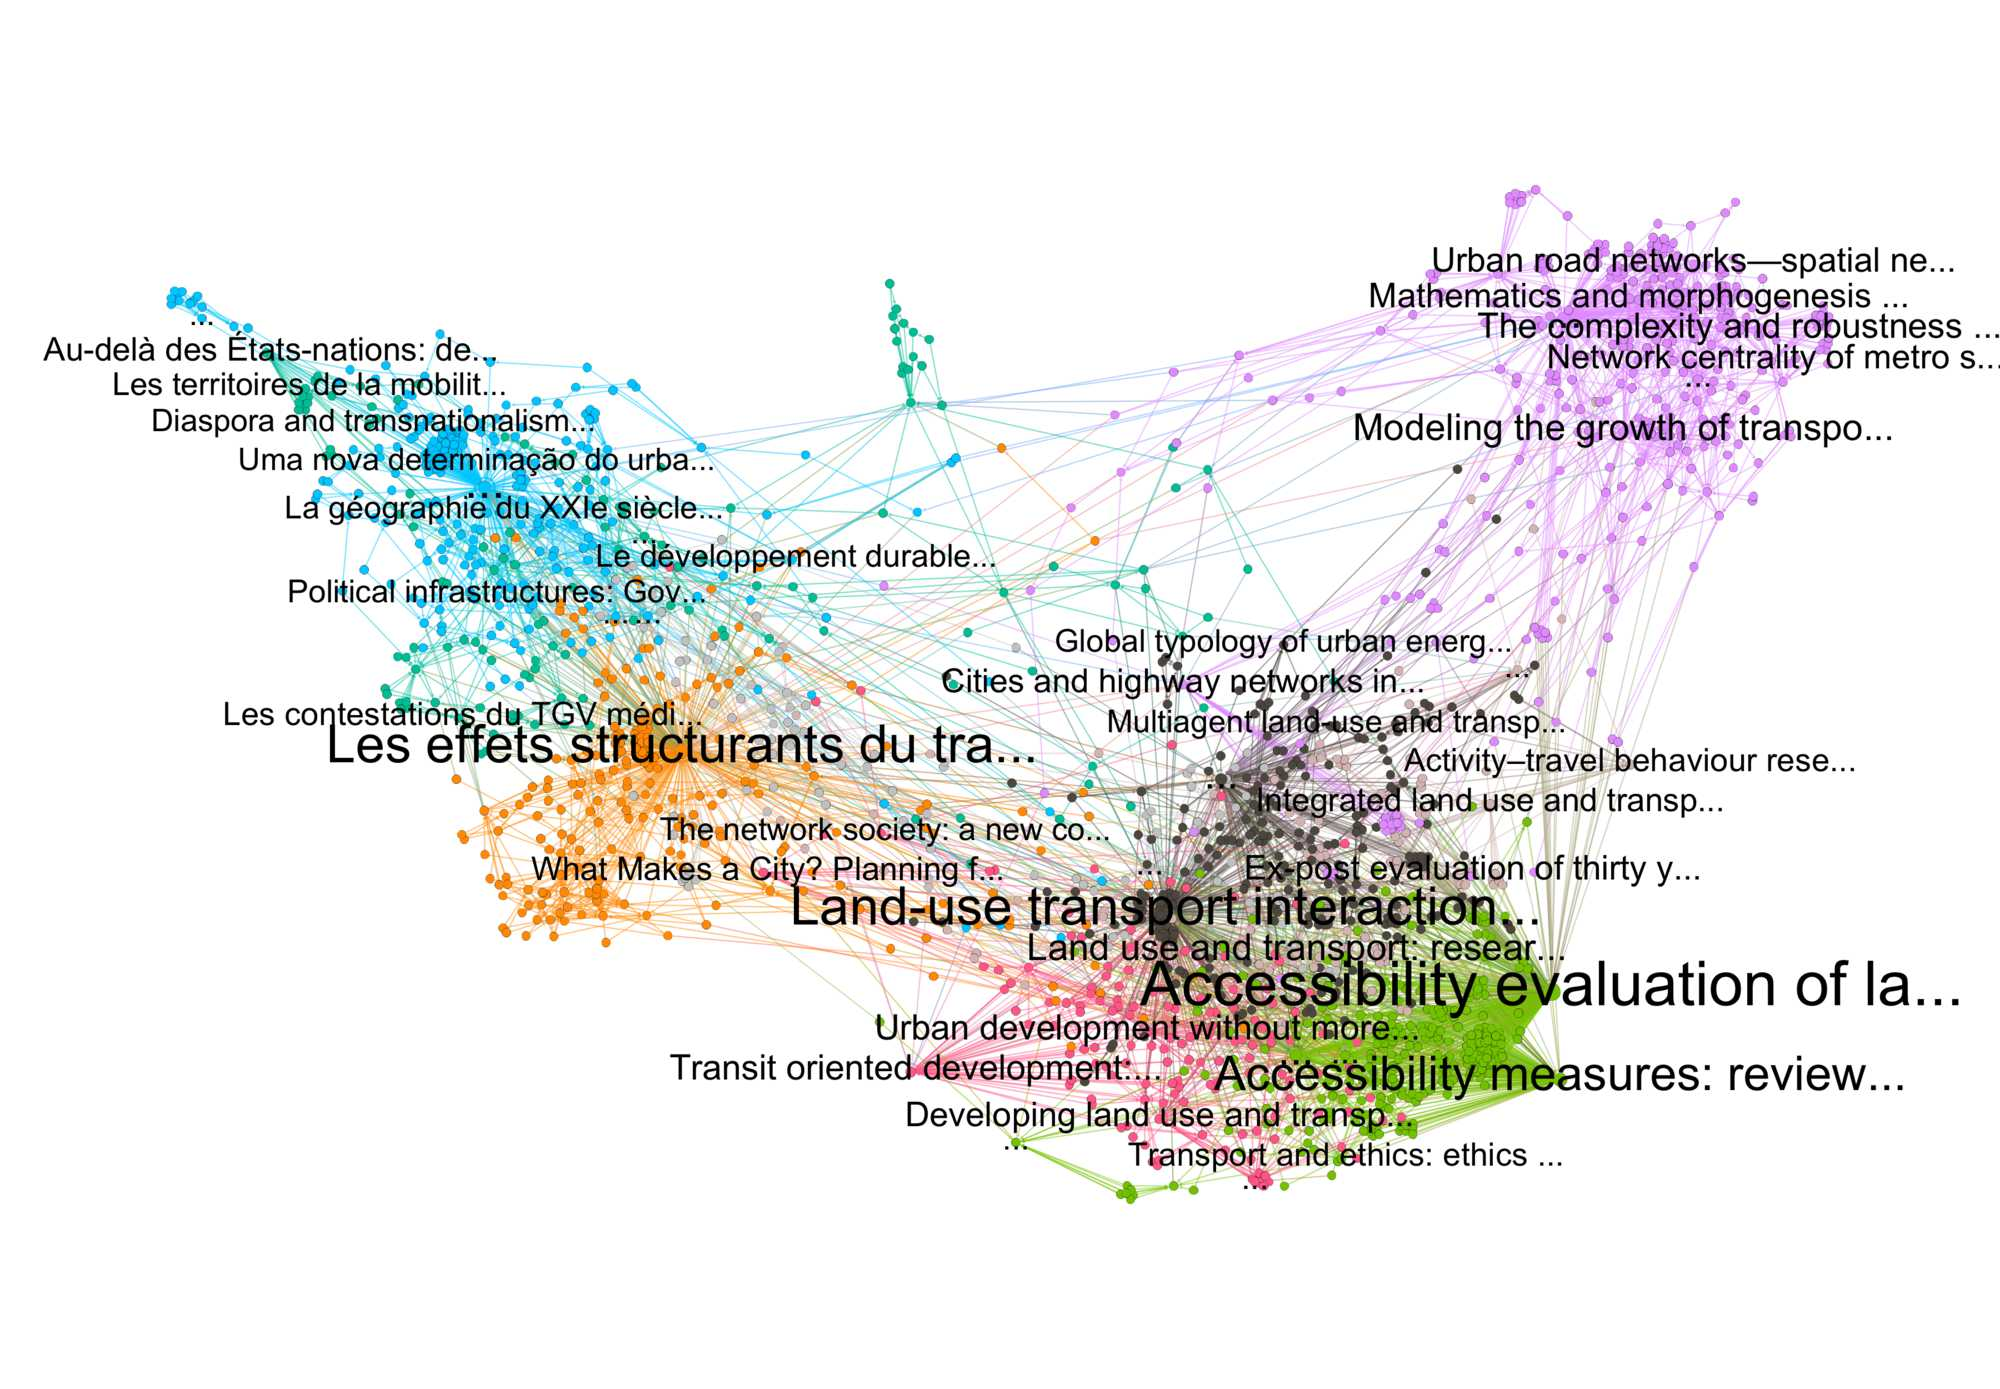
\includegraphics[width=0.9\textwidth,trim={0 2cm 0 2cm},clip]{figures/2-2-2-fig-quantepistemo-citnw.jpg}	
\end{center}

\medskip

\tiny

\vspace{-1cm}

Raimbault, J. (2019). Exploration of an interdisciplinary scientific landscape. Scientometrics, 119(2), 617-641.

\nocite{raimbault2019exploration}

}

\sframe{Horizontal integration: model coupling}{

\begin{table}
\vspace{-0.5cm}
	\centering
	\begin{tabular}{|p{3.8cm}|p{3.5cm}|p{3.5cm}|}
	\hline
	\footnotesize
	& QUANT & SPENSER \\
	\hline
Time scale & 10 years & 40 years \\
Spatial scale & UK & UK \\
Spatial resolution & MSOA & MSOA \\
Agent granularity & Aggregated counts & individual level \\
Static/Dynamic & Equilibrium (static) & Dynamic \\
Randomness & Deterministic & Monte-Carlo \\\hline
Transportation & 3 modes & NA \\
Economics & Accessibility-based relocations & NA \\
Demographics & NA & Data-driven \\
Migration flows & Accessibility-based relocations & Data-driven \\
\hline
	\end{tabular}
\end{table}

\smallskip

\footnotesize

\begin{itemize}
	\item Weak coupling Luti $\rightarrow$ microsimulation
	\item Weak coupling Microsimulation $\rightarrow$ Luti
	\item Strong coupling: as much choices as potential ``coupling processes''
	% iteration in time and/or during model iterations of interactions between inputs/outputs: \textit{using demographic output of QUANT as the migration module of SPENSER - i.e. replacing the SIMIM module}  \textit{using demographic output of SPENSER as input of QUANT - useful to ``run QUANT in the future''}

\end{itemize}

}


\sframe{Horizontal integration: multi-modeling}{


\begin{center}
\frame{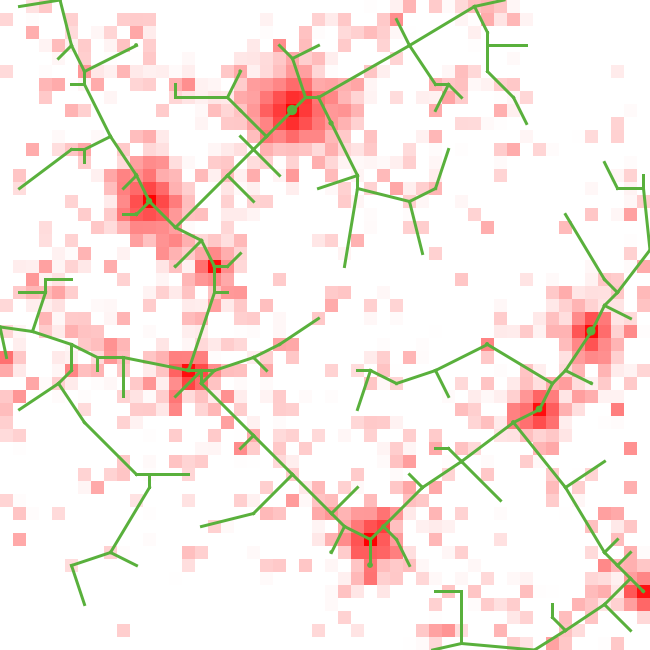
\includegraphics[width=0.28\textwidth]{figures/coevol_example_nw-connection}}\hspace{0.1cm}
\frame{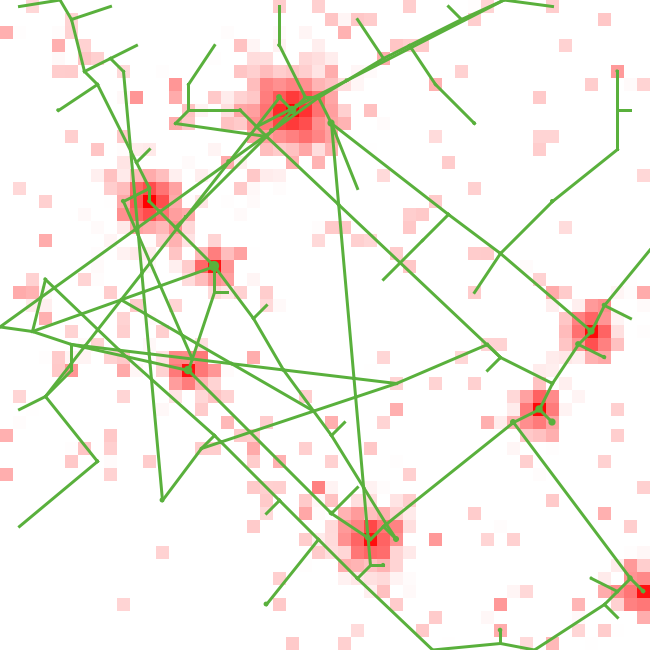
\includegraphics[width=0.28\textwidth]{figures/coevol_example_nw-random}}\hspace{0.1cm}
\frame{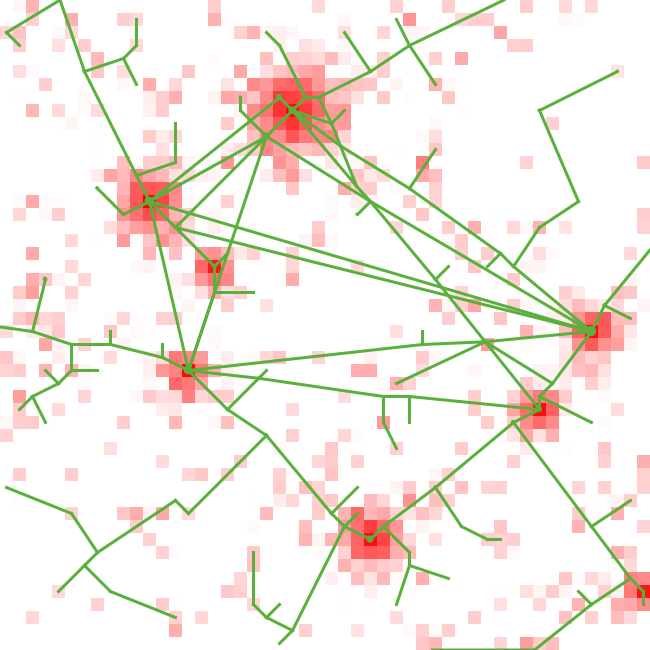
\includegraphics[width=0.28\textwidth]{figures/coevol_example_nw-gravity}}\\\vspace{0.1cm}
\frame{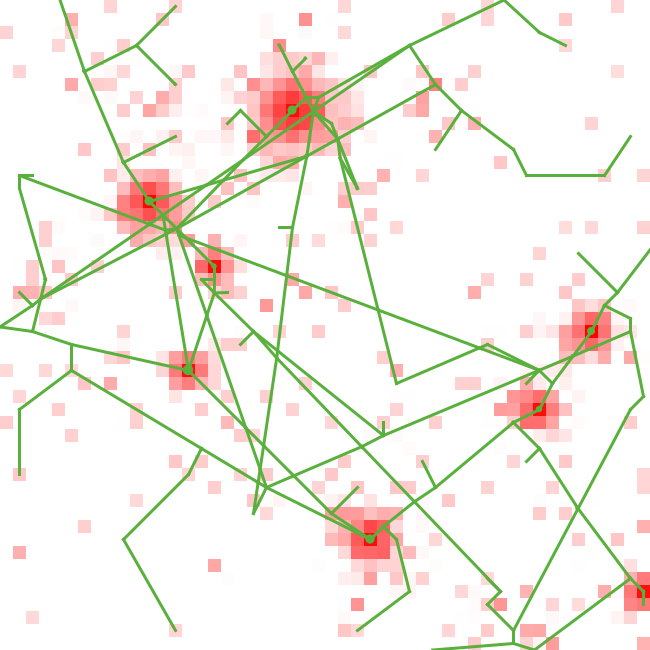
\includegraphics[width=0.28\textwidth]{figures/coevol_example_nw-rndbrkdwn}}\hspace{0.1cm}
\frame{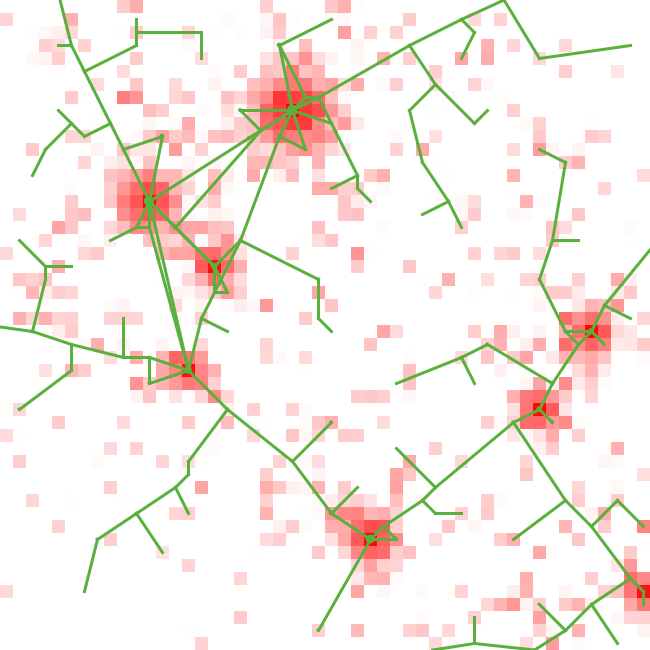
\includegraphics[width=0.28\textwidth]{figures/coevol_example_nw-cost}}\hspace{0.1cm}
\frame{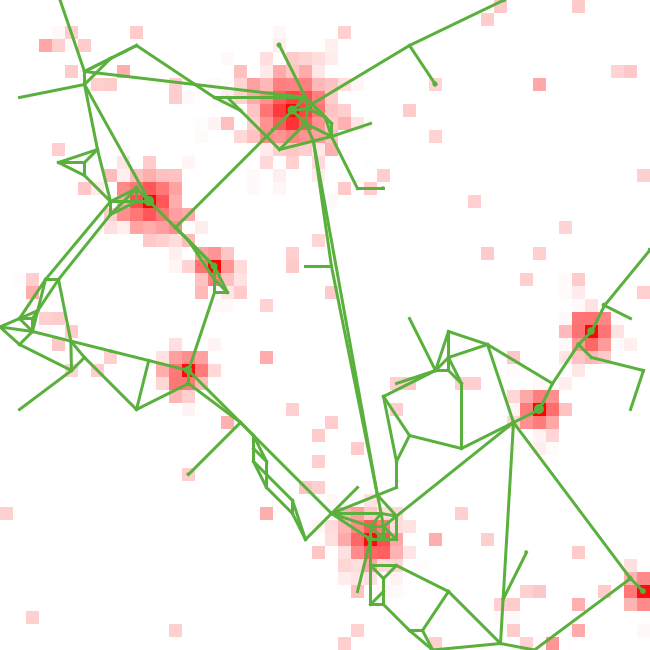
\includegraphics[width=0.28\textwidth]{figures/coevol_example_nw-bio}}
\end{center}


%\footnotesize\textit{In order: connection; random; deterministic breakdown; random breakdown; cost-driven; biological.}

\medskip

\tiny

Raimbault, J. (2018). Multi-modeling the morphogenesis of transportation networks. In Artificial Life Conference Proceedings (pp. 382-383). MIT Press, Cambridge.

\nocite{raimbault2018multi}


}

\sframe{Vertical integration: multi-scale models}{


\textit{Processes specific to scales, coupling implies dedicated ontologies} 

%\cite{raimbault2019towards}

\bigskip

\begin{center}
	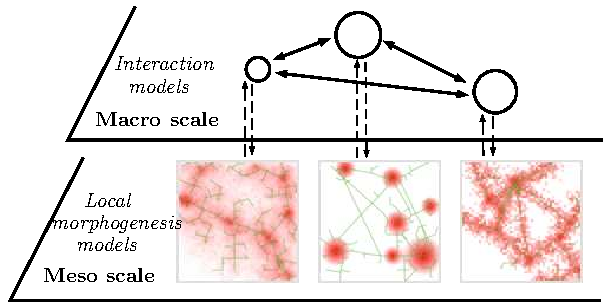
\includegraphics[width=0.9\textwidth]{figures/multiscale_morph.pdf}
\end{center}


}


\sframe{Towards knowledge integration: ERC Geodivercity}{

% presentation generale de Geodivercity

\begin{columns}
\begin{column}{0.4\textwidth}
	\centering
	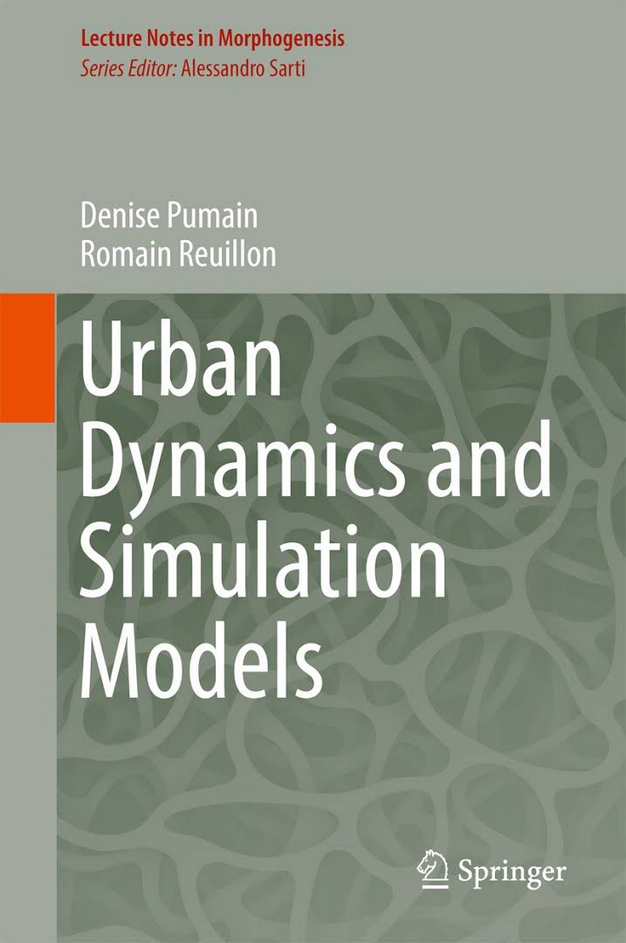
\includegraphics[width=0.9\textwidth]{figures/urban-dynamics-simulation-models-geodivercity.png}
\end{column}
\begin{column}{0.6\textwidth}
	Development of evolutive urban theory
	
	 \nocite{pumain2018evolutionary}
	
	\medskip

	$\rightarrow$ Recurrent stylized facts on main systems of cities
	
	$\rightarrow$ Construction of simulation models (with an explicative purpose)
	
	$\rightarrow$ Tools and methods to explore simulation models
	
	\smallskip
	
	
\includegraphics[width=\textwidth]{figures/openmole.png}
		
	
\end{column}
\end{columns}

\bigskip
\tiny

Pumain, D. (2018). An evolutionary theory of urban systems. In International and Transnational Perspectives on Urban Systems (pp. 3-18). Springer, Singapore.


}


\sframe{Iterative construction of knowledge across domains}{


\begin{center}
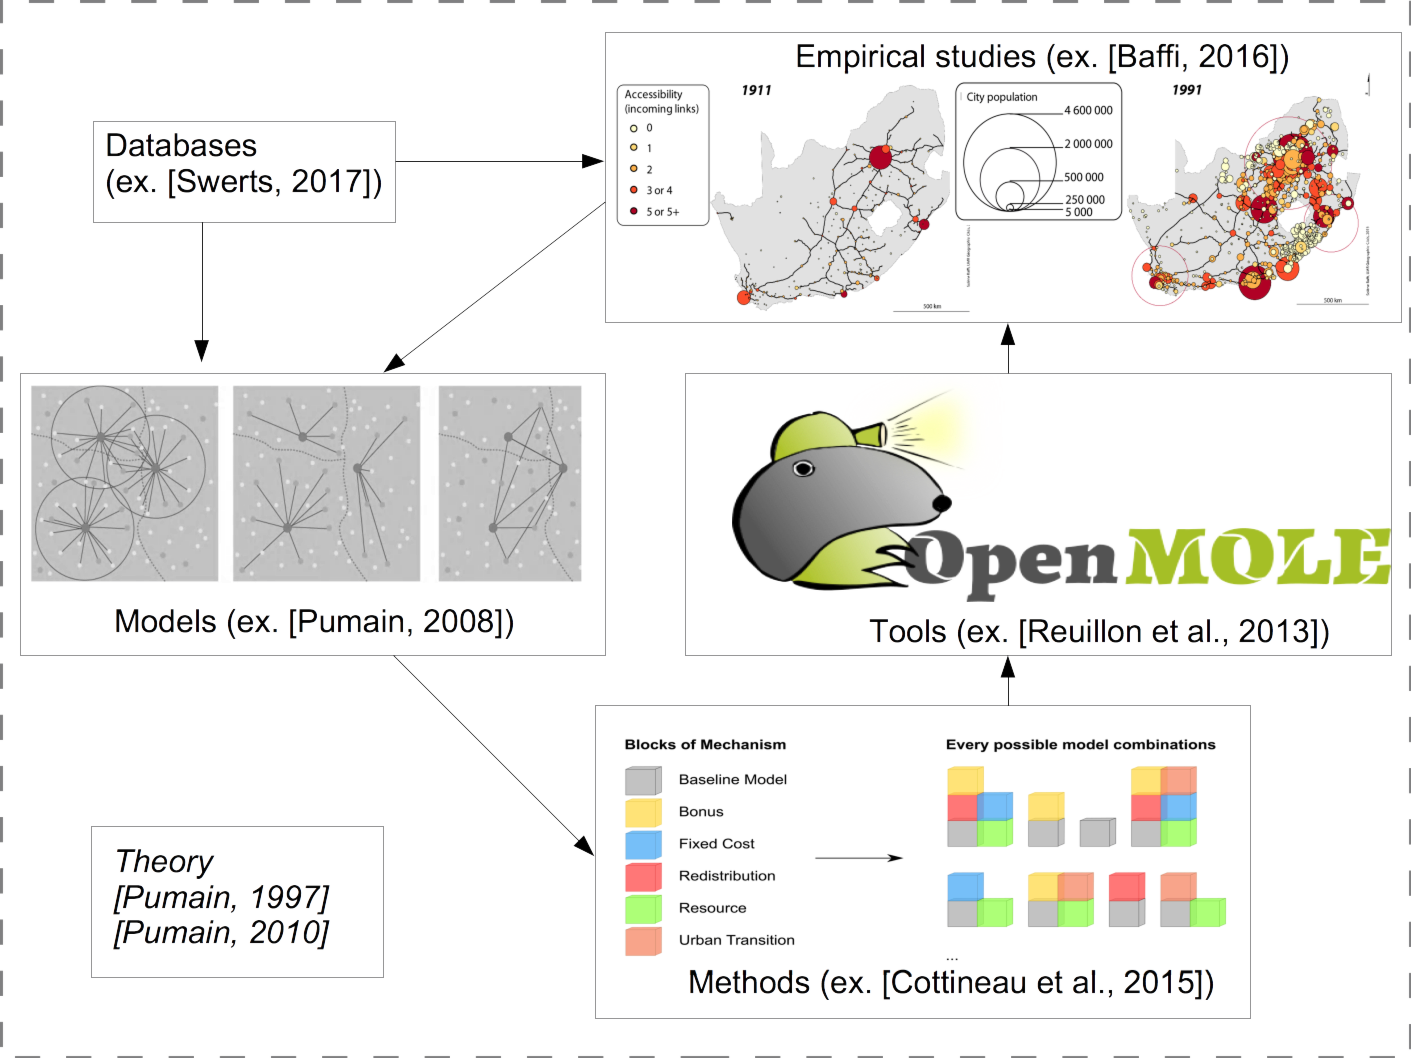
\includegraphics[height=0.75\textheight]{figures/openmoleslide}
\end{center}

\medskip

\tiny

Raimbault, J. (2017). An Applied Knowledge Framework to Study Complex Systems. In Complex Systems Design \& Management (pp. 31-45).

\nocite{raimbault2017applied}


\nocite{baffi:tel-01389347}
\nocite{pumain2008socio}
\nocite{reuillon2013openmole}
\nocite{cottineau2015modular}
\nocite{swerts2017database}
\nocite{pumain1997pour}
\nocite{pumain2010theorie}

}



\sframe{Model exploration methods to foster knowledge integration}{
	
	\textit{(i) Innovative exploration methods; (ii) Scaling of methods on high performance computing environments; (iii) No interference with the model.}
	
	\smallskip
	
	\centering
	
	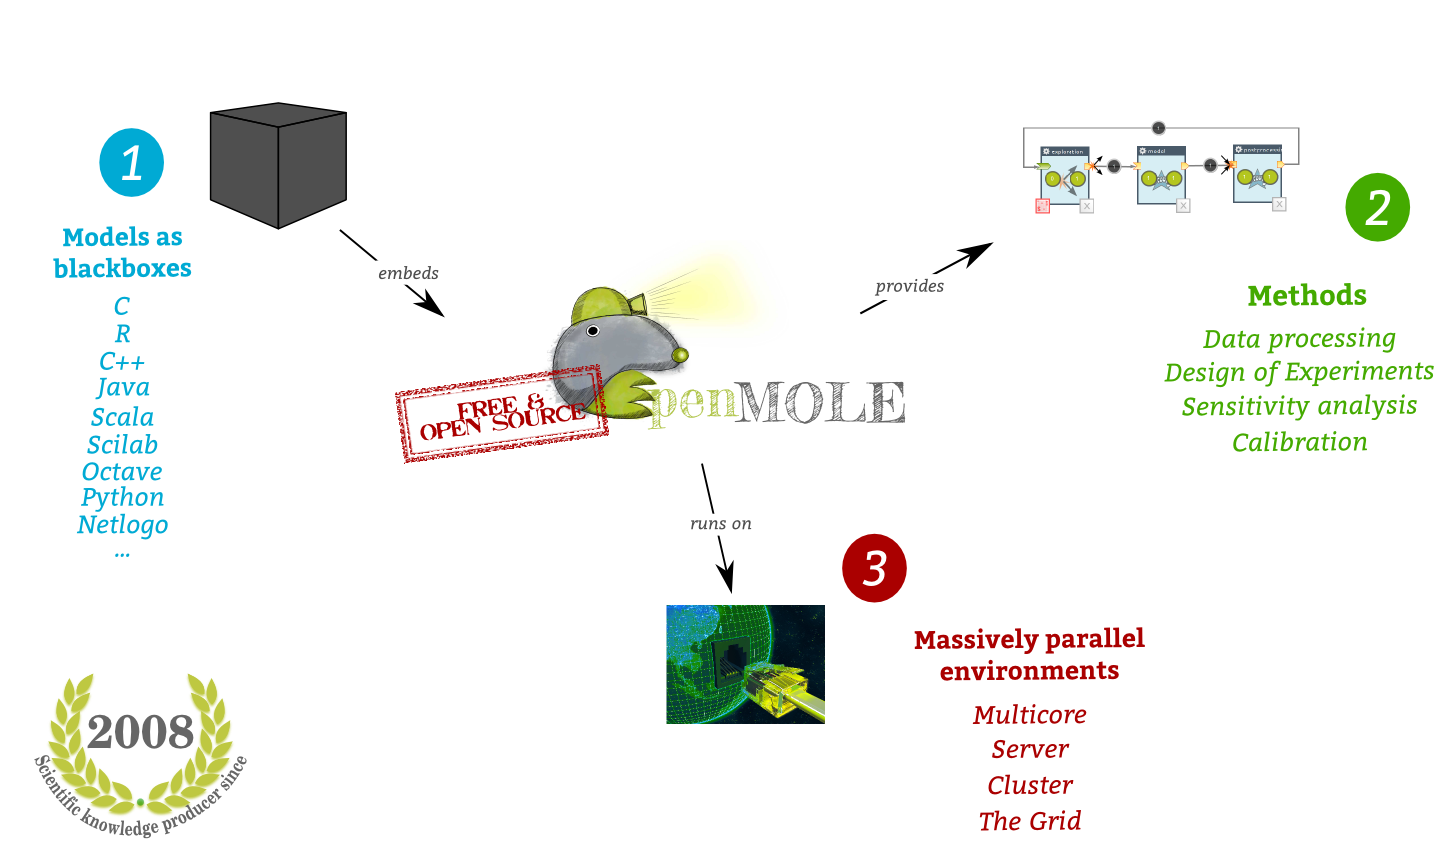
\includegraphics[width=\textwidth]{figures/openmoleGal.png}
	
}


\sframe{New methods for spatial models}{

\begin{columns}
	\begin{column}{0.5\textwidth}
	
		\justify
	
		\textit{Variance-based method to assess the sensitivity of agent-based models to spatial configuration}
		
		\bigskip
		
		\begin{center}
			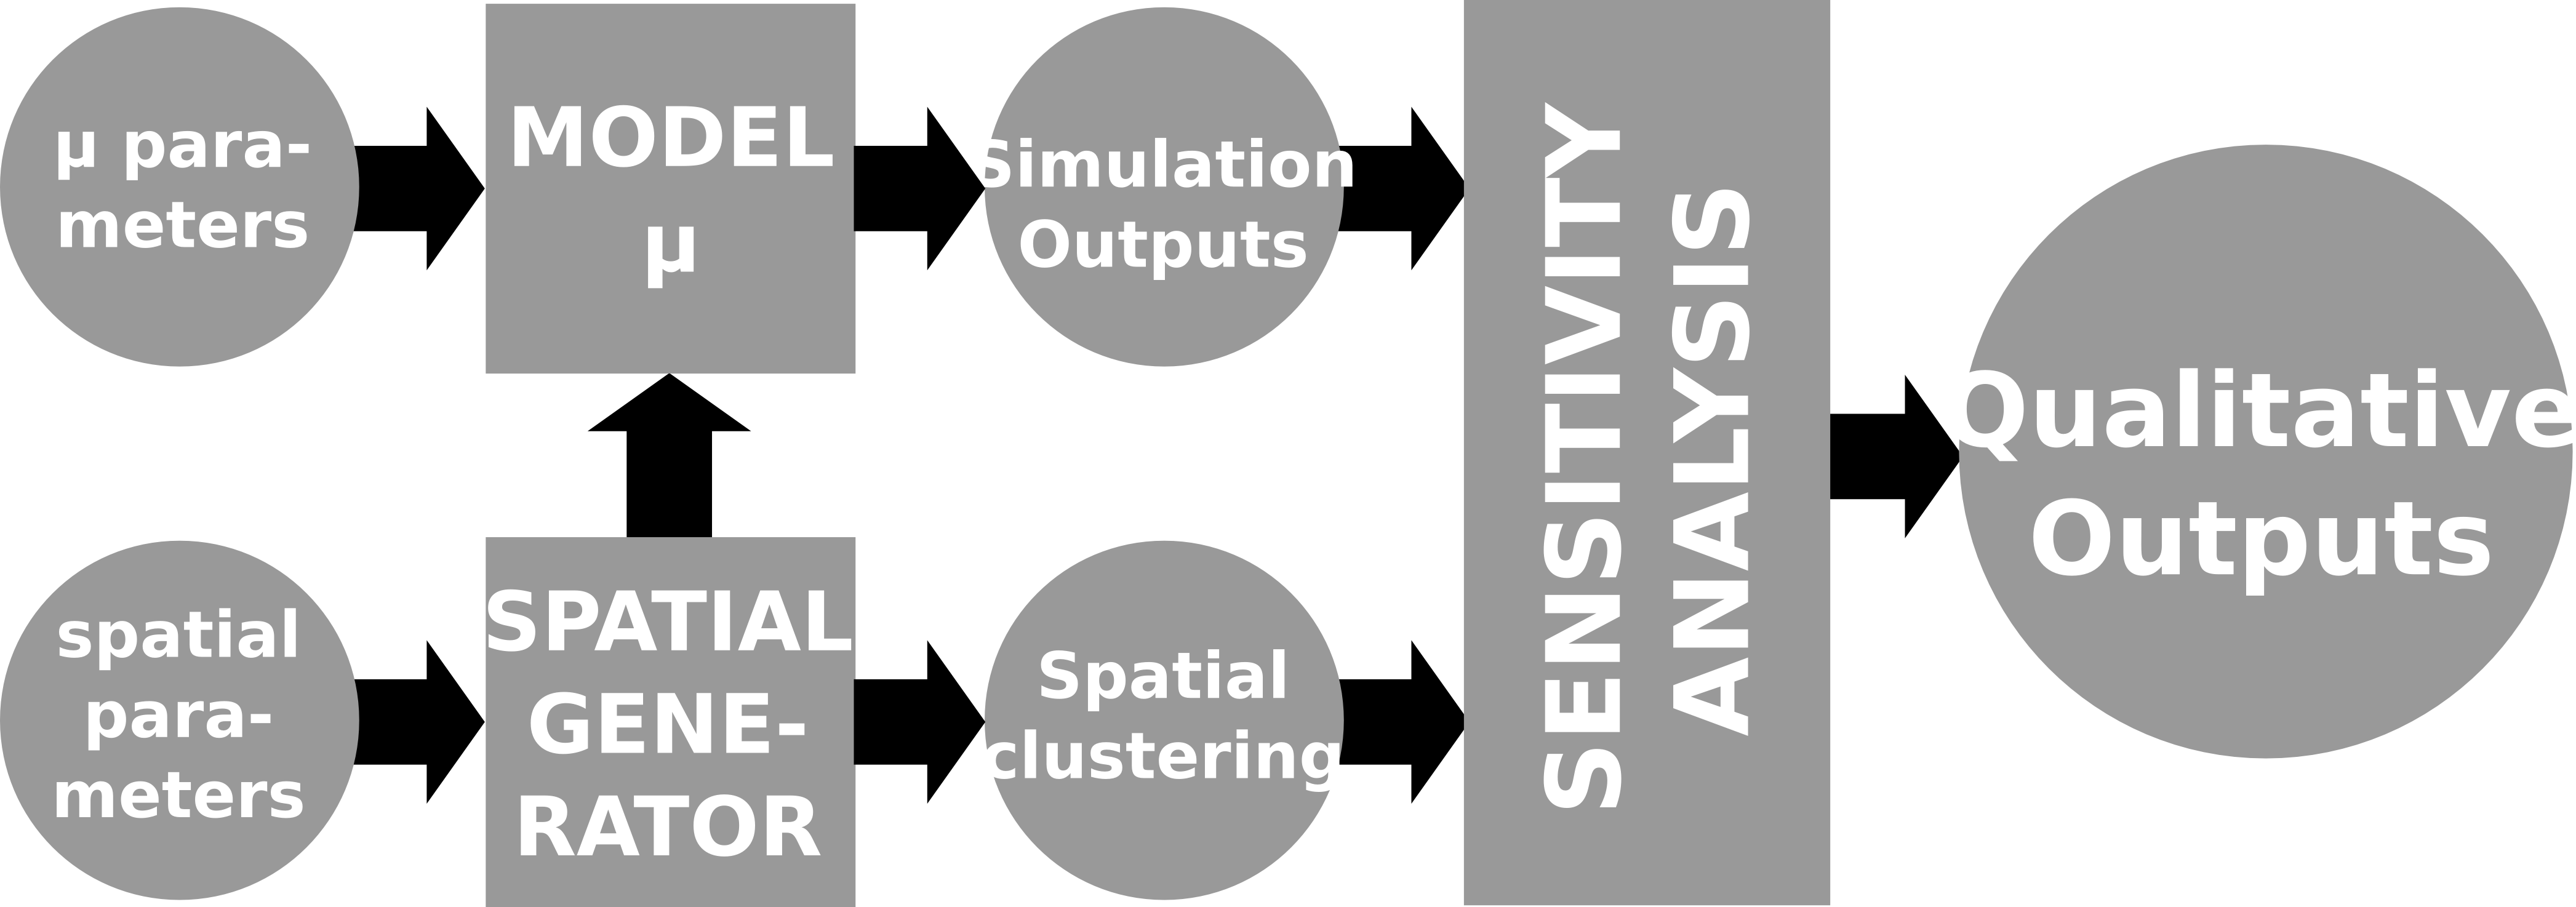
\includegraphics[width=\textwidth]{figures/spatialsens_spacemattersworkflow.png}
		\end{center}

		\tiny
		
		Raimbault, J., Cottineau, C., Texier, M. L., Néchet, F. L., \& Reuillon, R. (2018). Space Matters: extending sensitivity analysis to initial spatial conditions in geosimulation models. arXiv preprint arXiv:1812.06008.
		
	\end{column}
	\vrule{}
	\begin{column}{0.5\textwidth}

	\justify
	
	\textit{Generators of synthetic spatial configurations}

	\bigskip

		\begin{center}
			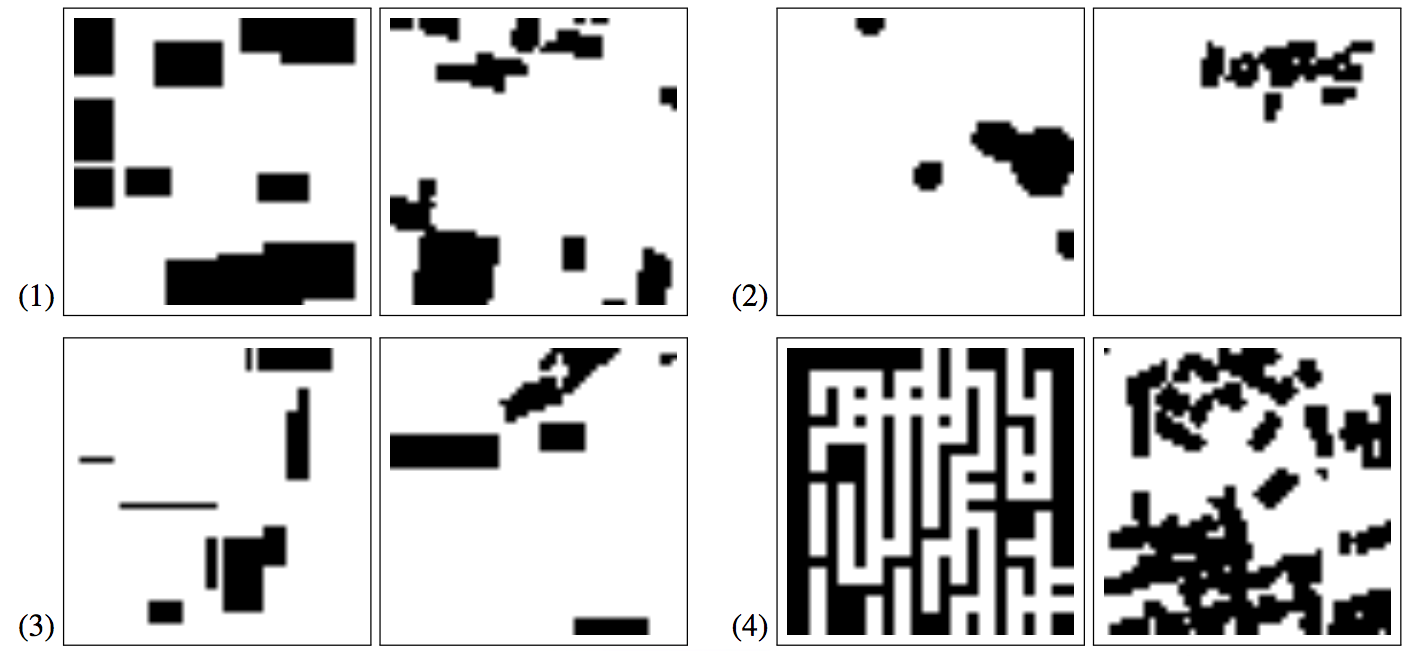
\includegraphics[width=\textwidth]{figures/spatialsens_calib.png}
		\end{center}

			\tiny 
			
			Raimbault, J. and Perret, J., 2019. Generating urban morphologies at large scales. \textit{Forthcoming in proceedings of Artificial Life 2019.} arXiv:1903.06807

	\end{column}

	
\end{columns}


}




\sframe{Towards models for sustainable policies}{

\textit{Benchmark of growth models for systems of cities} 

\nocite{raimbault2018systematic}

\centering

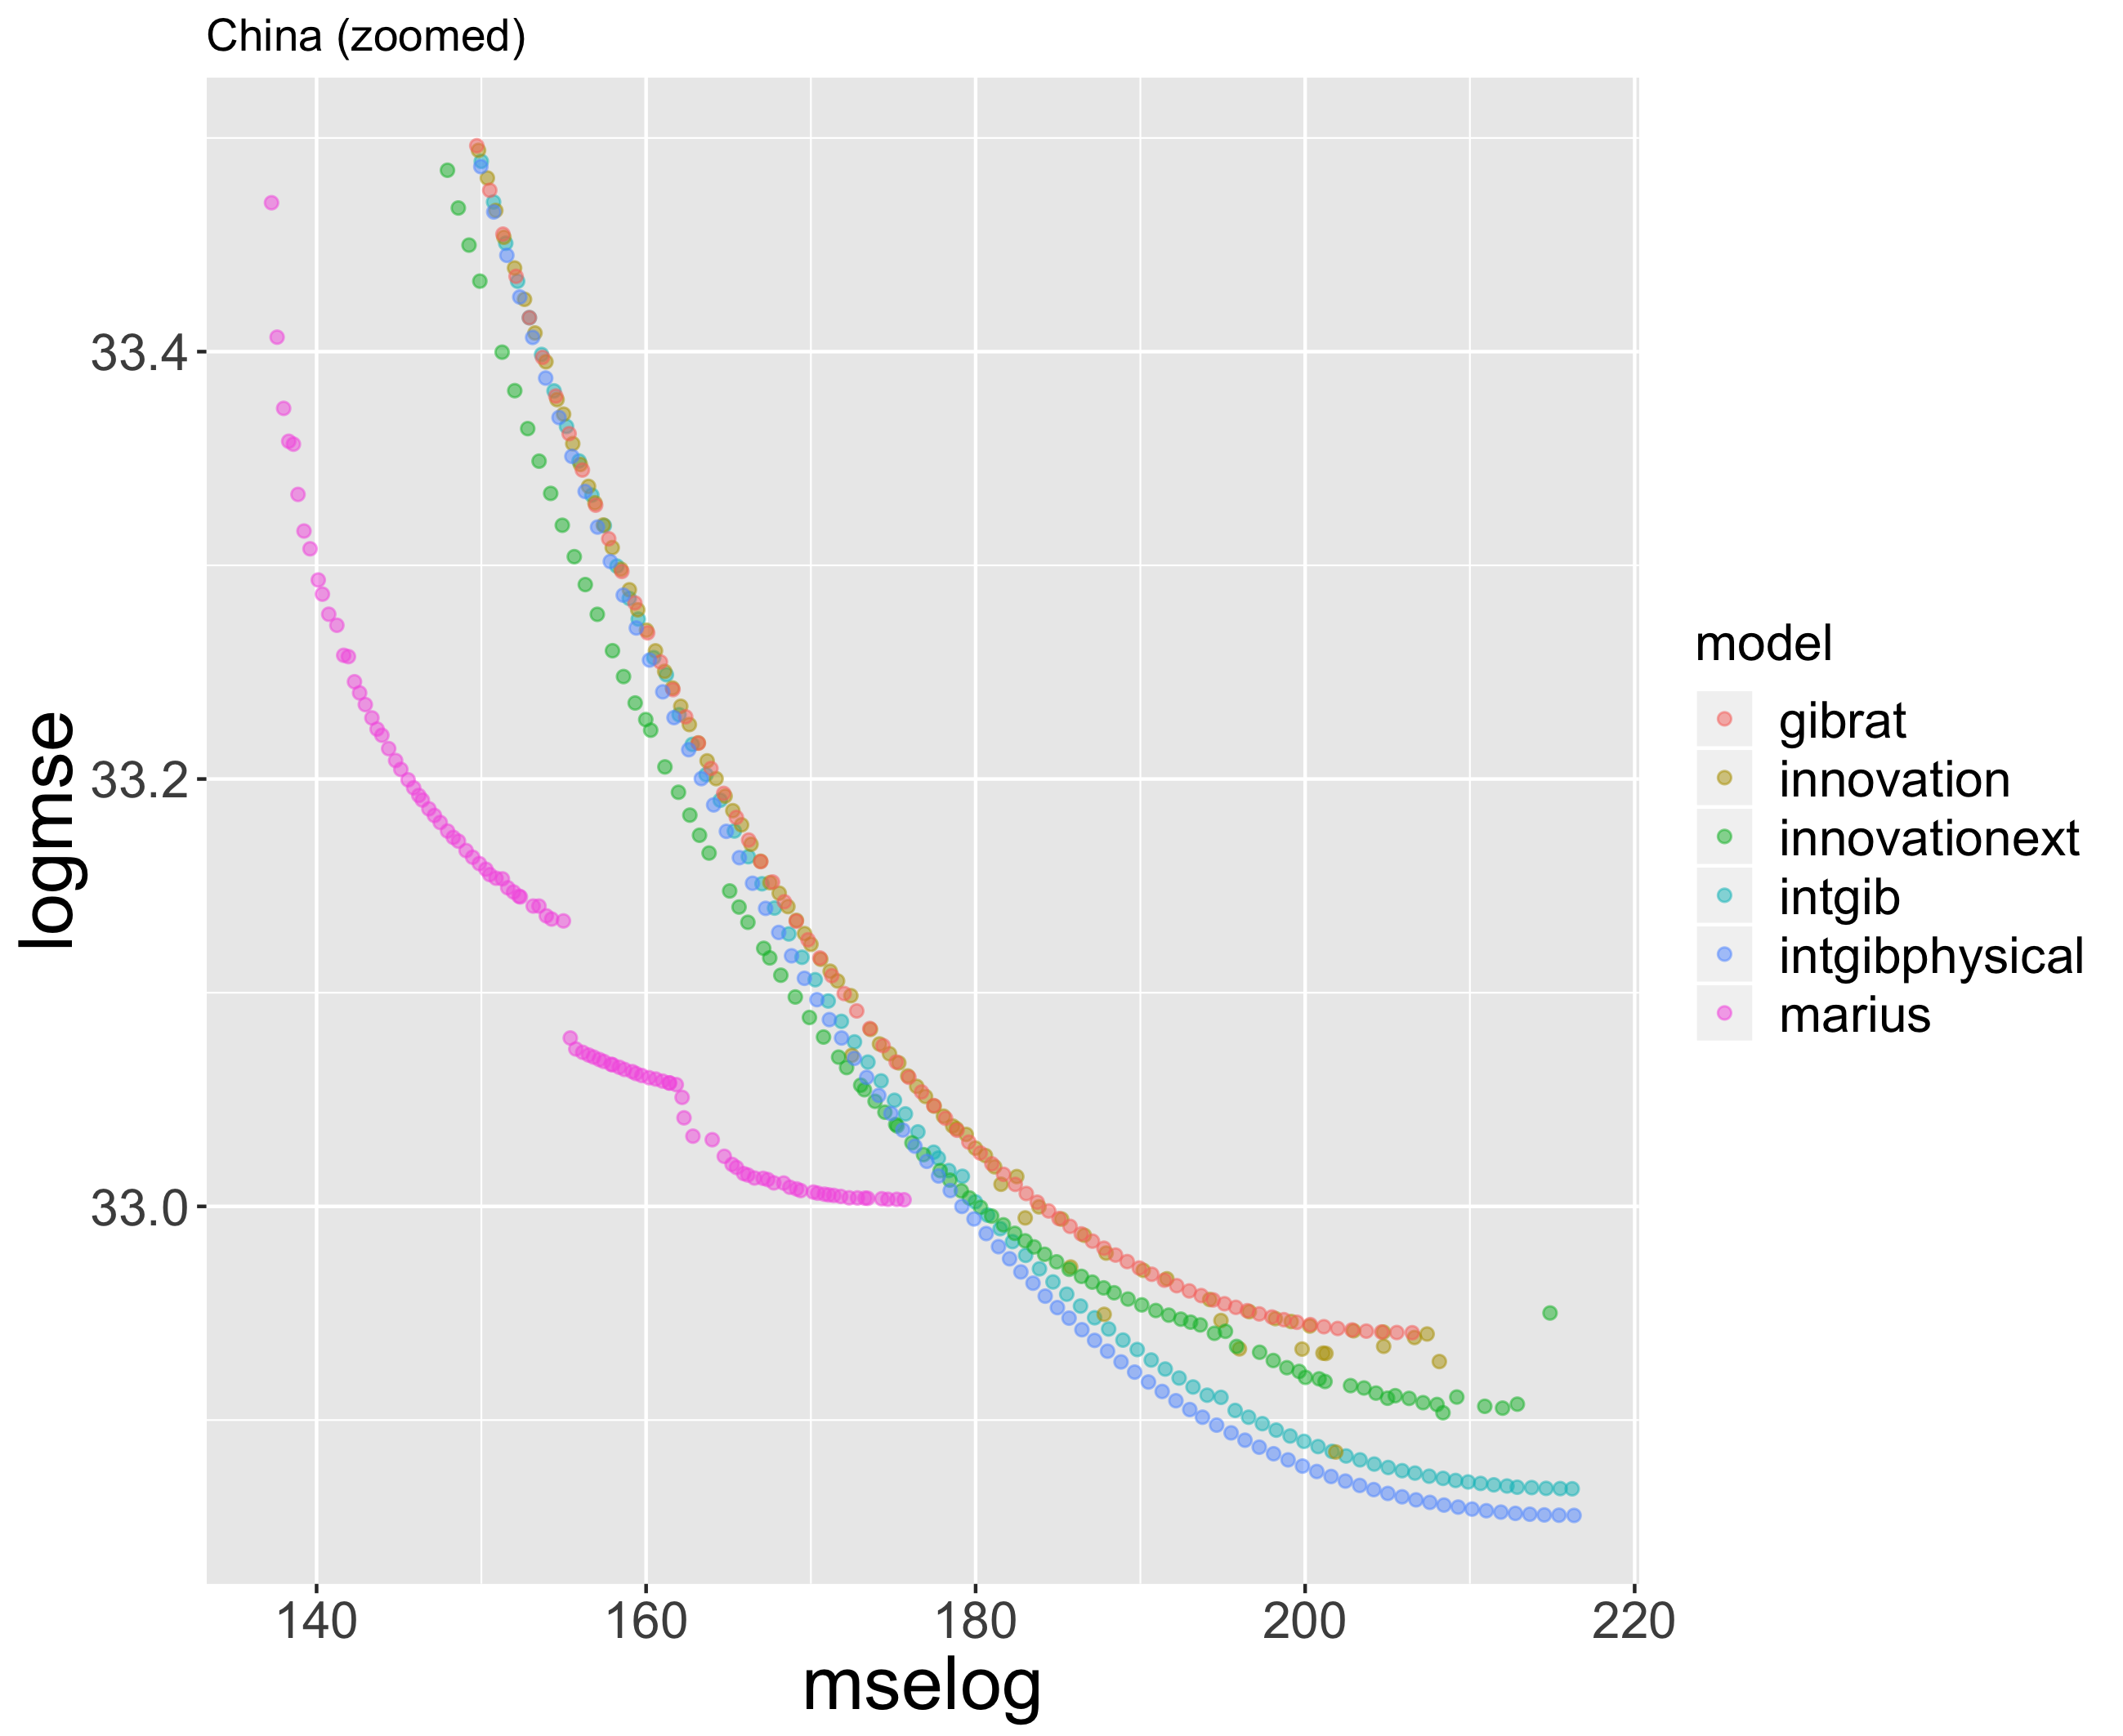
\includegraphics[width=0.85\textwidth]{figures/CN_zoomed.png}

}


\sframe{Towards models for sustainable policies}{

\textit{Identifying endogenous sustainable mega-city regions in Europe}

\medskip

% Marami
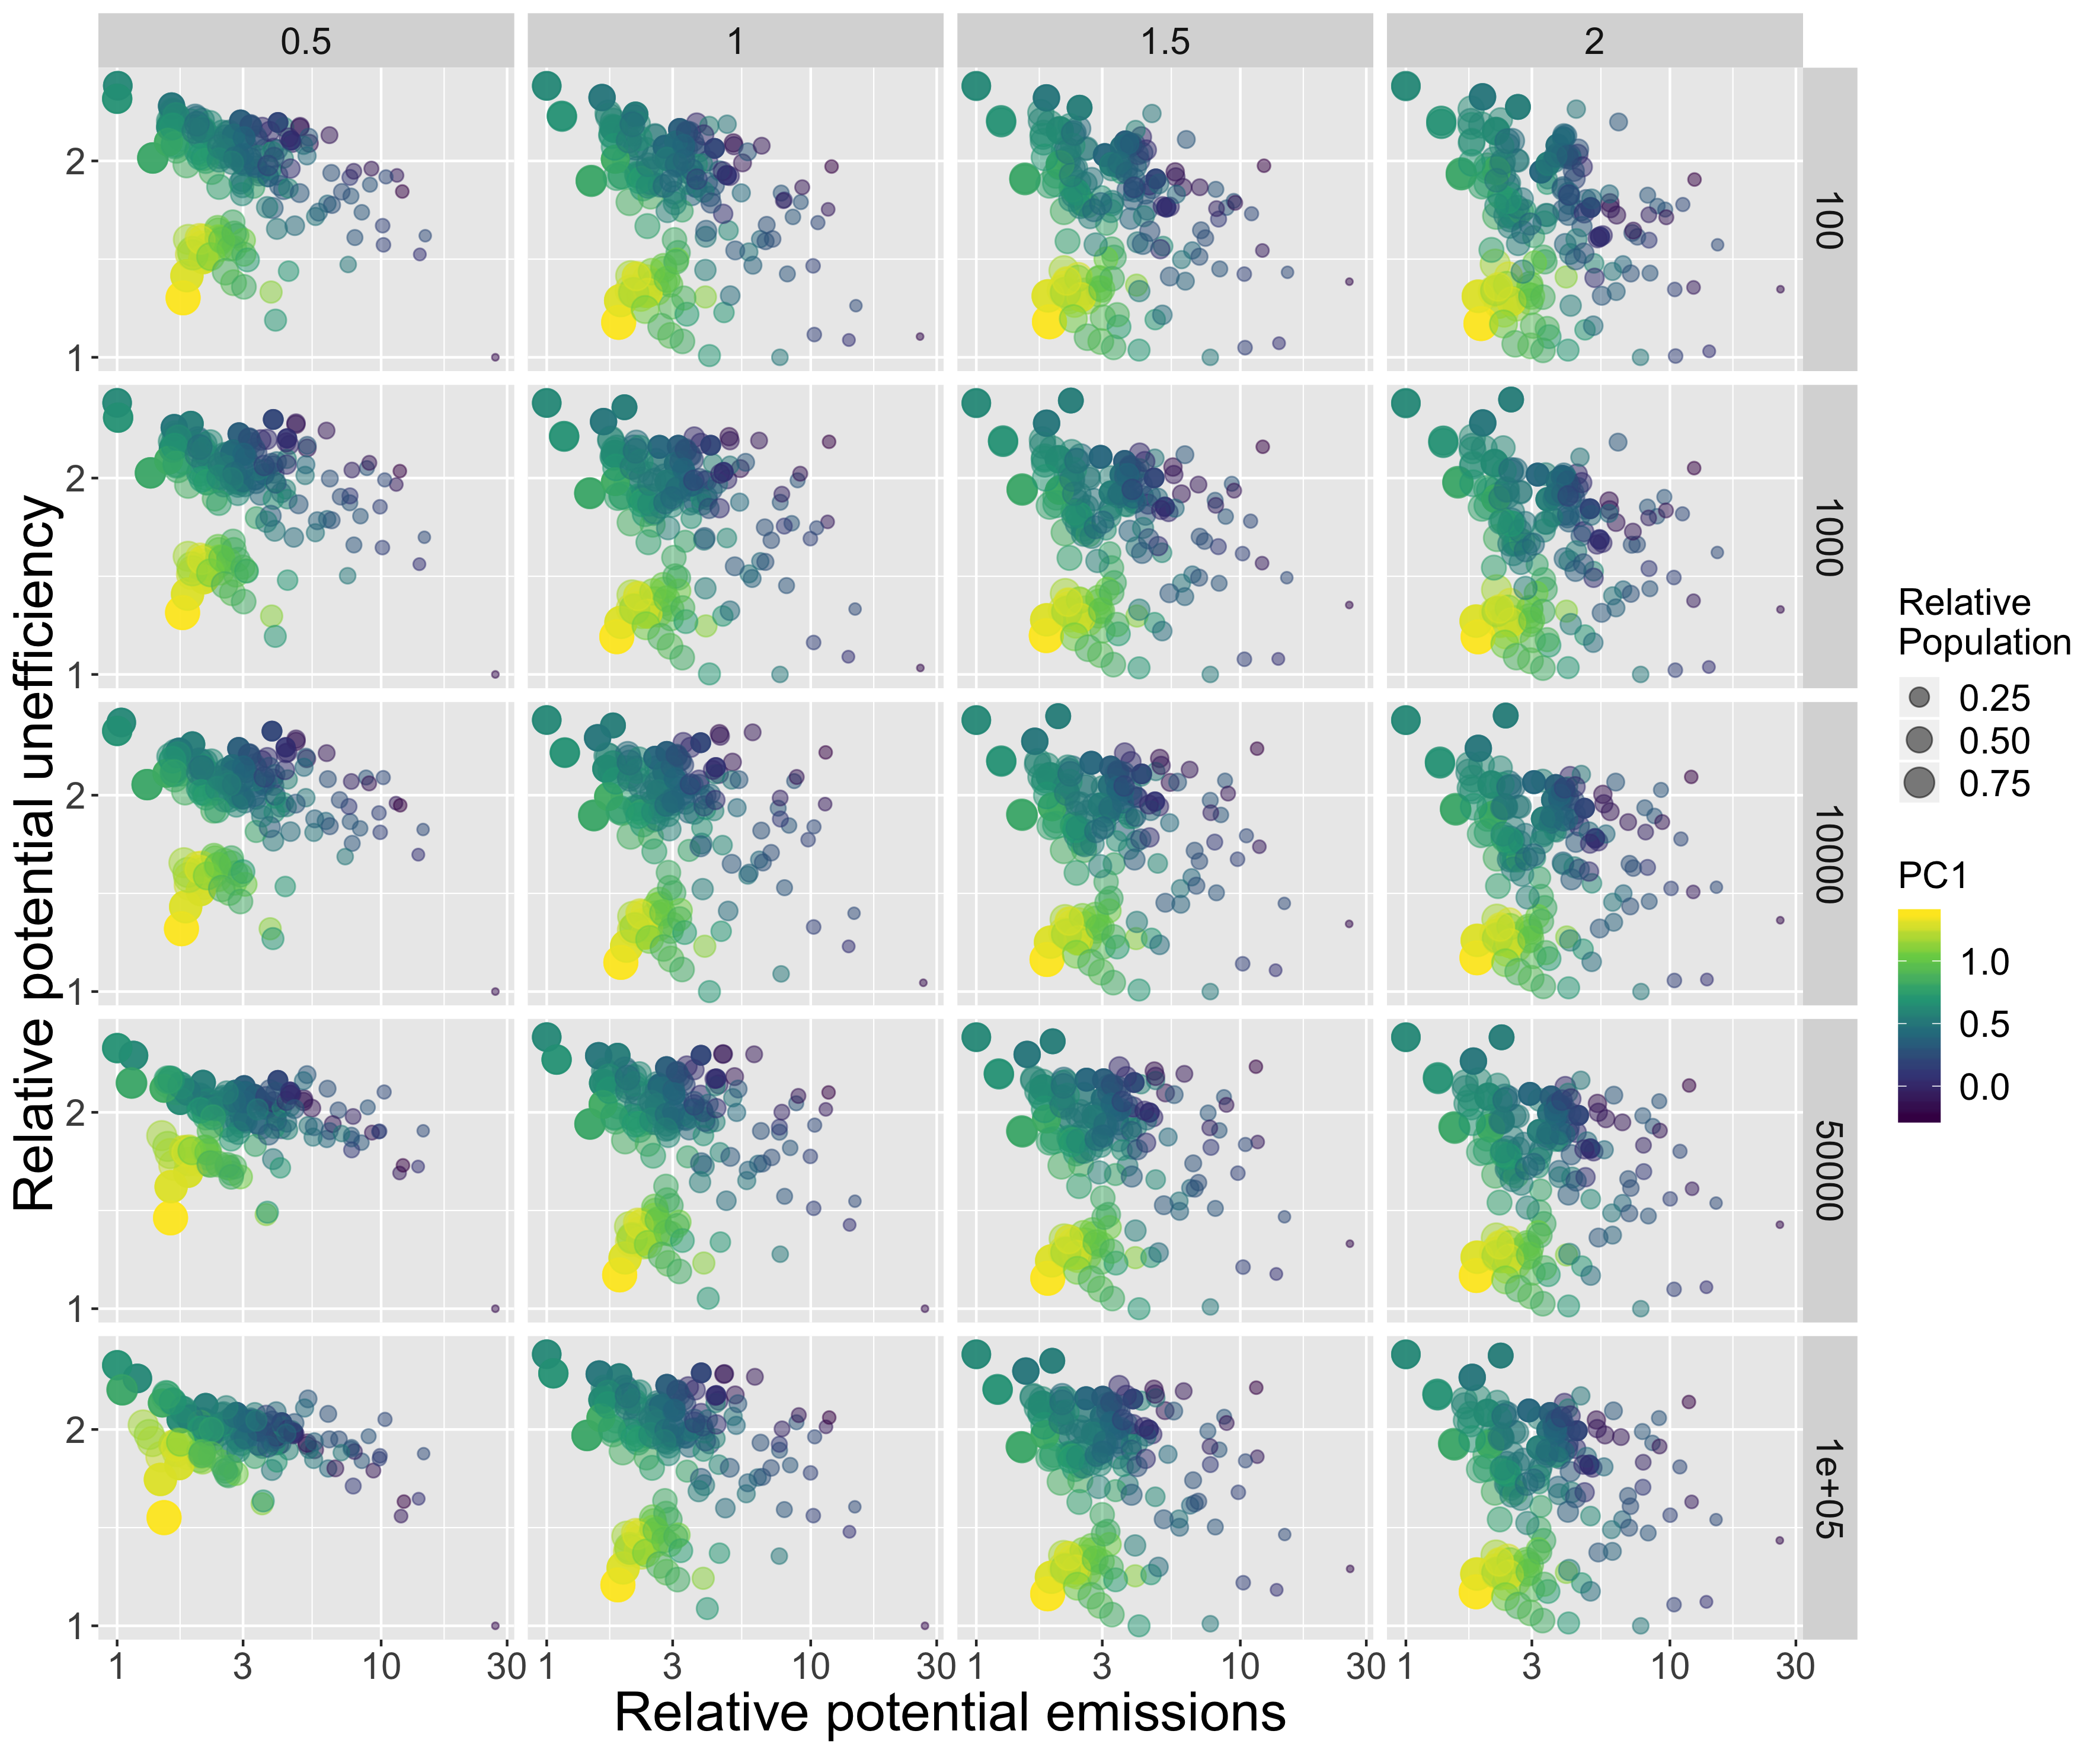
\includegraphics[width=0.49\textwidth]{figures/aggreg_morpho_relemissions-relefficiency_colpc1_logscale.png}
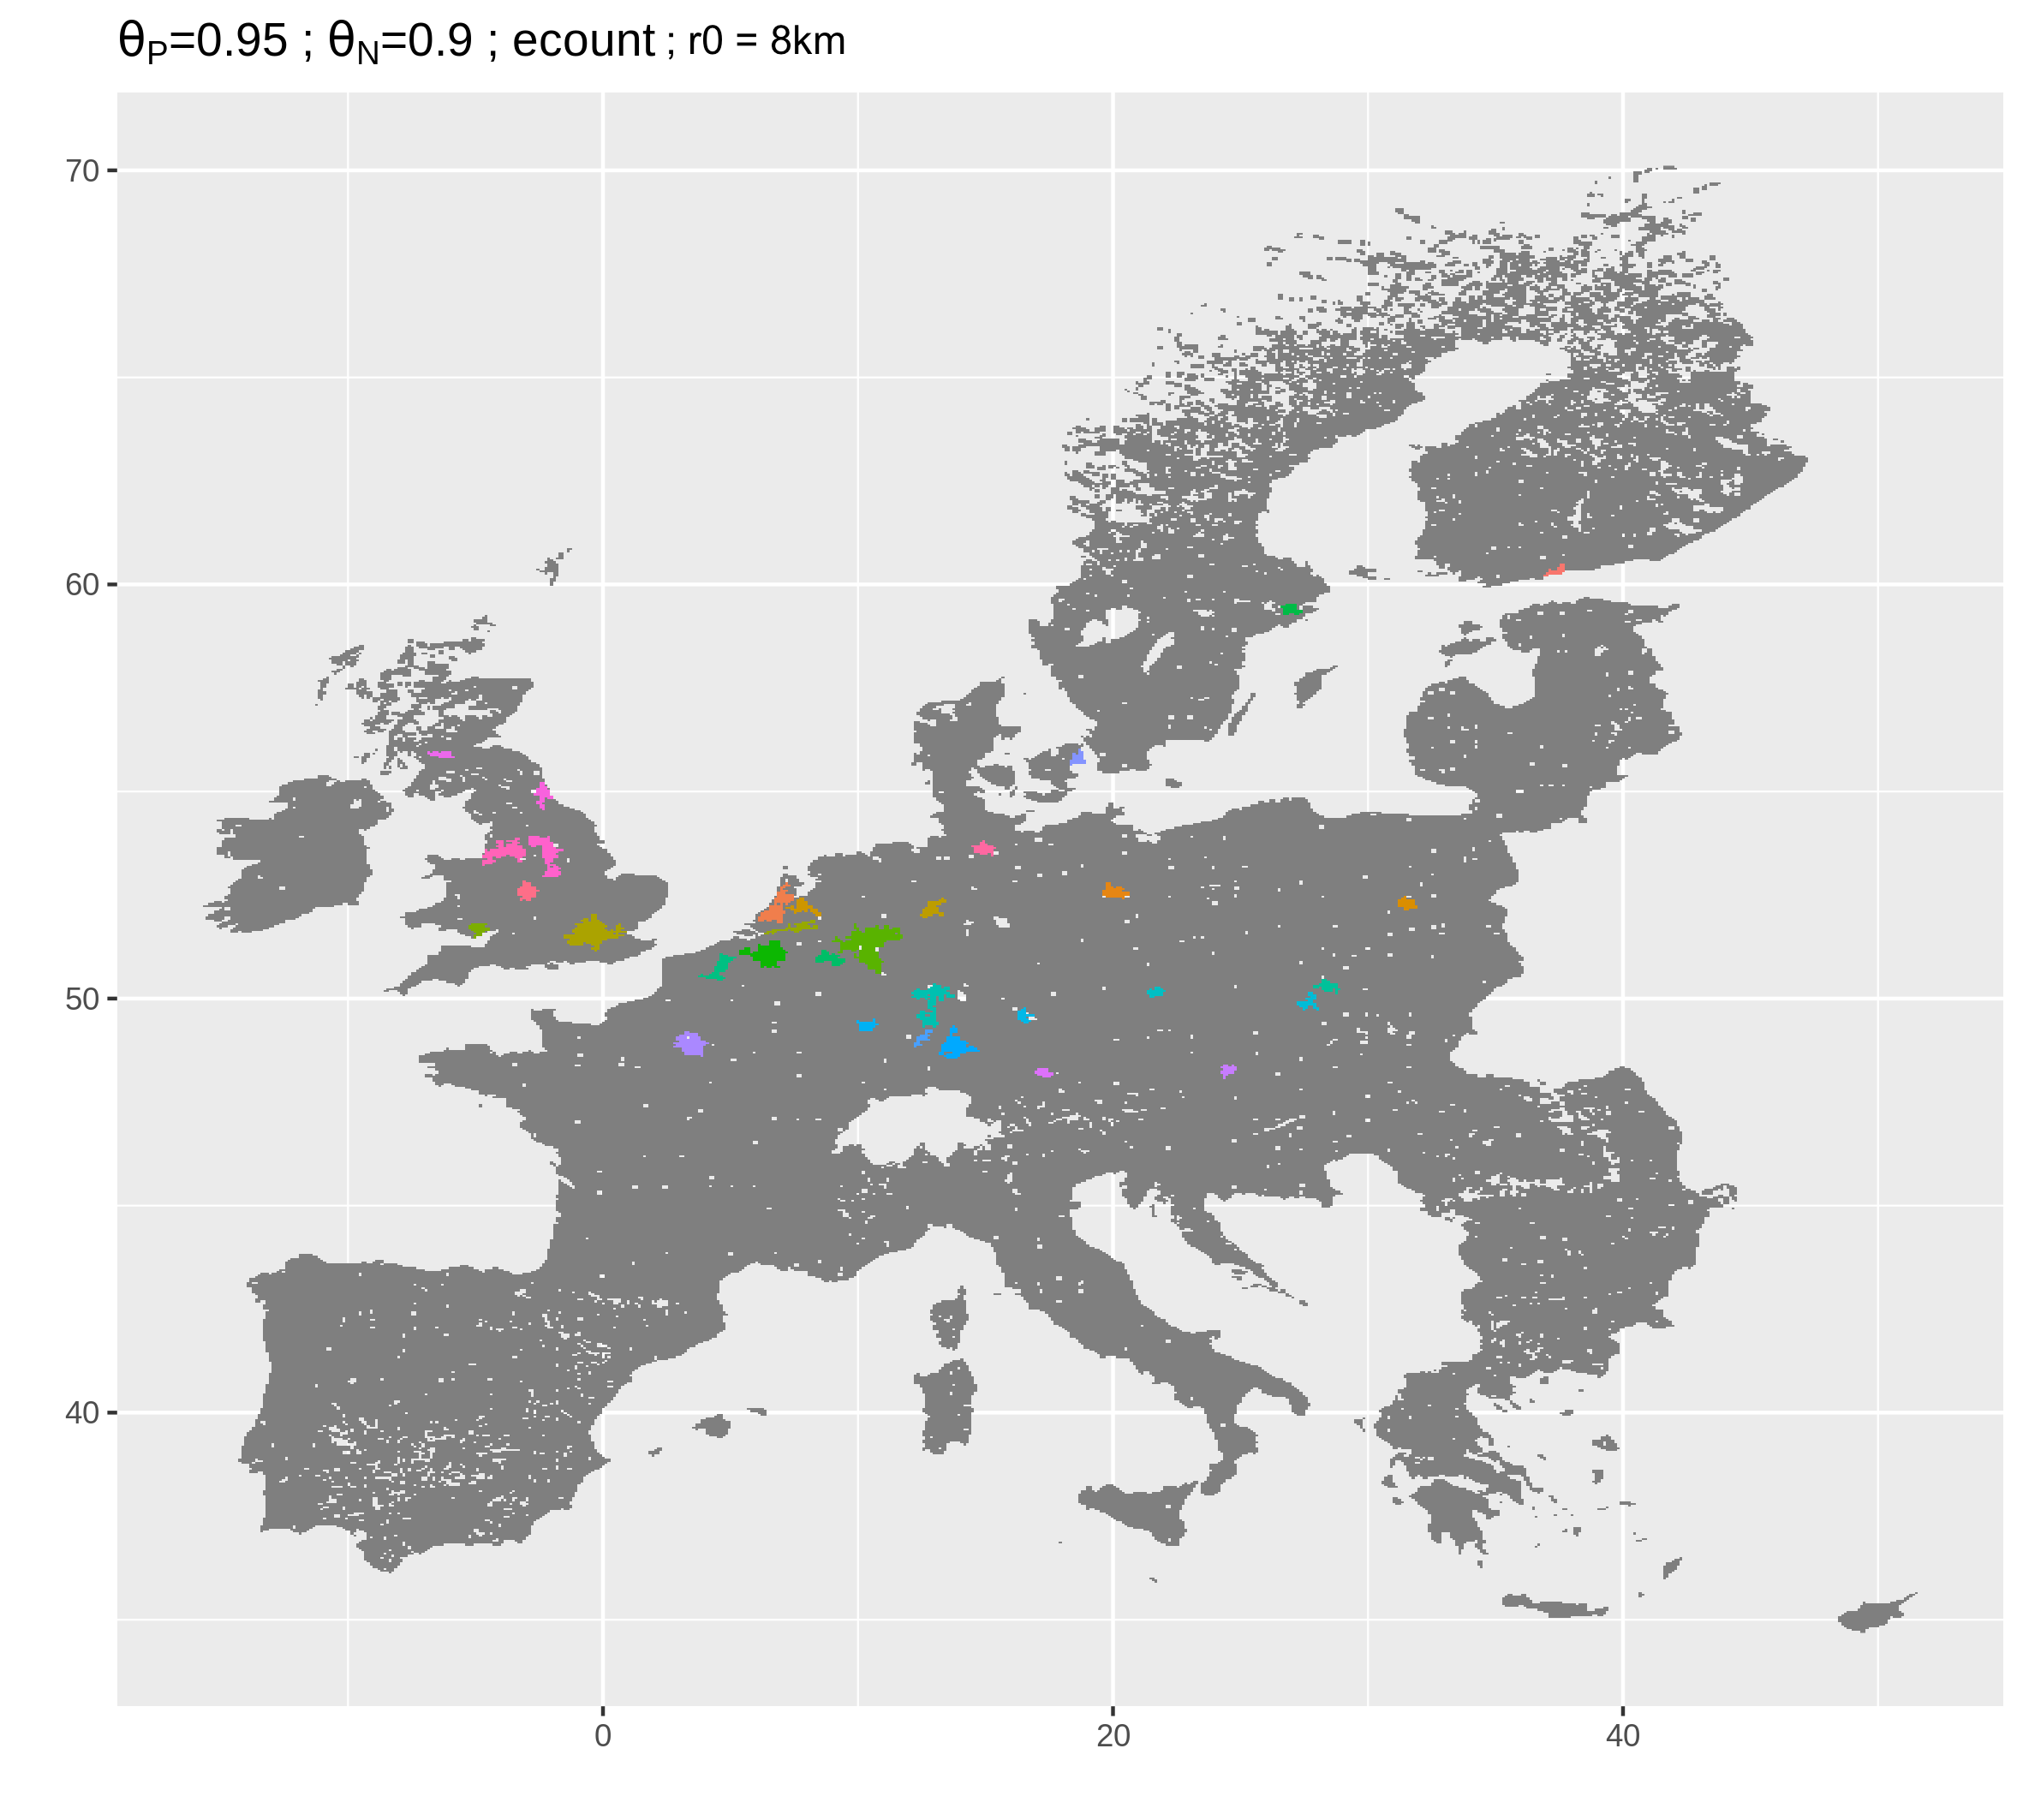
\includegraphics[width=0.49\textwidth]{figures/totalPop4183694_00056402_ecount850_radius8000.png}

\tiny

\bigskip

Raimbault, J. (2019). Multi-dimensional Urban Network Percolation. arXiv preprint arXiv:1903.07141.

}







\sframe{Conclusion}{

\justify

$\rightarrow$ Multiple ways to model urban systems: \textbf{towards more interdisciplinary coupling and comparison of models.}

\smallskip

$\rightarrow$ At which scale? \textbf{Towards multi-scale models.}

\smallskip

$\rightarrow$ With complementary aspects of knowledge? \textbf{Need for knowledge domain integration.}


\bigskip

\textbf{To use OpenMOLE (free and open software) and contribute: }\\
\url{next.openmole.org}

\bigskip


%
\textbf{Some references}

\medskip

\tiny

%
%
%\medskip


%Raimbault, J. (2018). Caract{\'e}risation et mod{\'e}lisation de la co-{\'e}volution des r{\'e}seaux de transport et des territoires (Doctoral dissertation, Université Paris 7 Denis Diderot). \url{https://halshs.archives-ouvertes.fr/tel-01857741}

Raimbault, J. (2017). An Applied Knowledge Framework to Study Complex Systems. In Complex Systems Design \& Management (pp. 31-45). arXiv:1706.09244.

\smallskip

Raimbault, J. (2018). Indirect evidence of network effects in a system of cities. Environment and Planning B: Urban Analytics and City Science, 2399808318774335.

\smallskip

Raimbault, J. (2018). Calibration of a density-based model of urban morphogenesis. PloS one, 13(9), e0203516.

\smallskip

Raimbault, J. (2019). An urban morphogenesis model capturing interactions between networks and territories. In The Mathematics of Urban Morphology (pp. 383-409). Birkhäuser, Cham.

\smallskip

Raimbault, J. (2019). Modeling the co-evolution of cities and networks. In Niel, Z., Rozenblat, C., eds. \textit{Handbook of Cities and Networks}, Edwar Elgar Publishing, \textit{in press}. arXiv:1804.09430



%
%
%
%
%%\smallskip
%
%%\textbf{Open repository} at \texttt{https://github.com/JusteRaimbault/UrbanGrowth}\\\smallskip
%%\textbf{Acknowledgments}: thanks to the \textit{EGI} for access to the infrastructure.
%
%
}
%
%

\sframe{Submit to special session at CCS}{


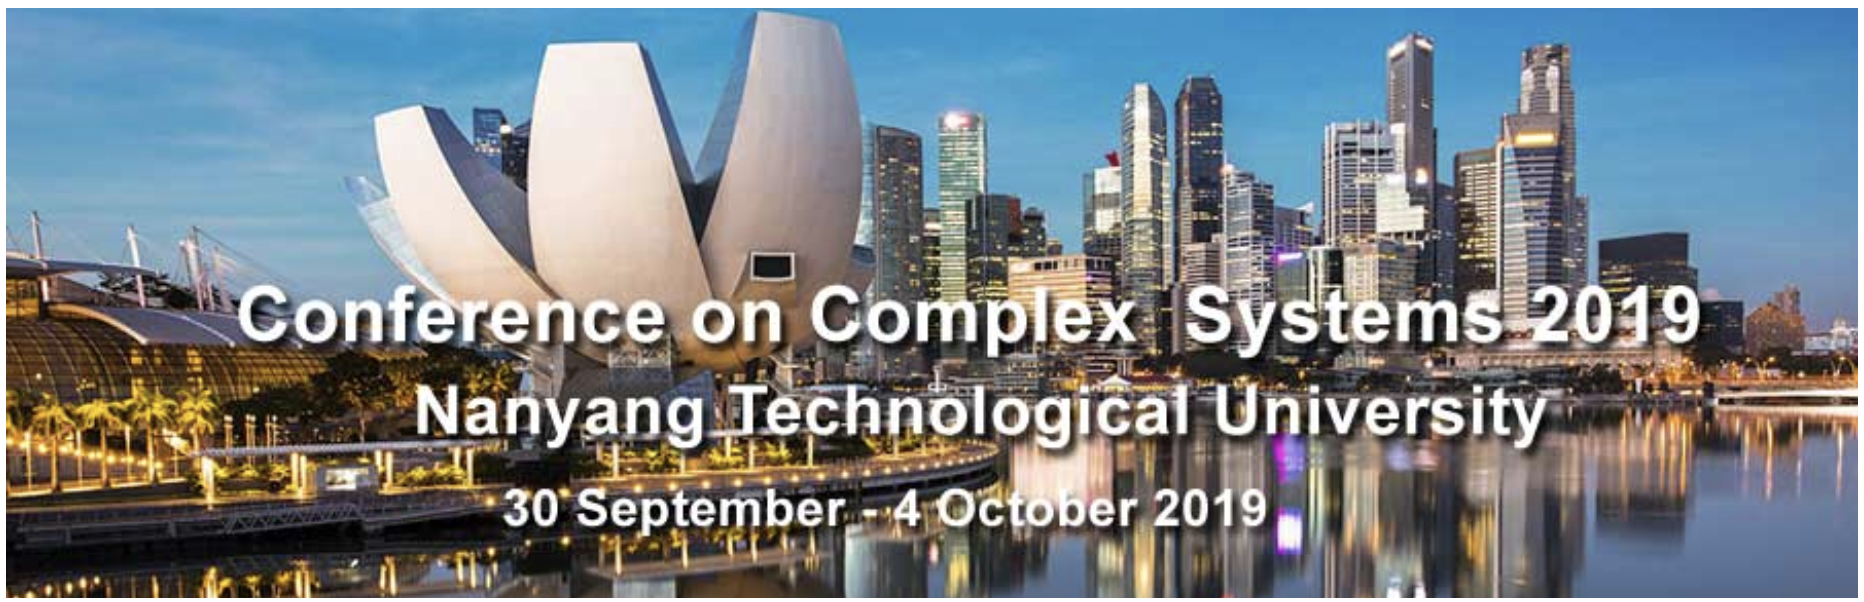
\includegraphics[width=\linewidth]{figures/ccs.png}

\medskip

\textit{Satellite session on methods and epistemology in modeling and simulation, at Conference on Complex Systems, 2nd October 2019}

\smallskip

\textbf{Submit your abstract before July 7th!}

\url{https://iscpif.fr/ccs-satelllite-session-2019-new-methods/}

\smallskip

\textbf{Submission link:}

\url{https://easychair.org/conferences/?conf=simexplo2019}

}




%%%%%%%%%%%%%%%%%%%%%
\begin{frame}[allowframebreaks]
\frametitle{References}
\bibliographystyle{apalike}
\bibliography{/Users/juste/ComplexSystems/CityNetwork/Biblio/Bibtex/CityNetwork,biblio}
\end{frame}
%%%%%%%%%%%%%%%%%%%%%%%%%%%%










\end{document}















